%---------------------------------------------------------------------
% This file provides a skeleton UCL DIS CDT report.
% \pdfinclusioncopyfonts=1
% This command may be needed in order to get \ell in PDF plots to appear. Found in
% https://tex.stackexchange.com/questions/322010/pdflatex-glyph-undefined-symbols-disappear-from-included-pdf
%---------------------------------------------------------------------
% Specify where ATLAS LaTeX style files can be found.
\newcommand*{\DISCDTLATEXPATH}{ucldiscdtlatex/latex/}
% Use this variant if the files are in a central location, e.g. $HOME/texmf.
%---------------------------------------------------------------------

\documentclass[NOTE, disdraft=false, UKenglish]{\DISCDTLATEXPATH UCLCDTDISdoc}
% The language of the document must be set: usually UKenglish or USenglish.
% british and american also work!
% Commonly used options:
%  cdtdraft=true|false   This document is an UCL CDT DIS draft.
%  paper=a4|letter       Set paper size to A4 (default) or letter.

%---------------------------------------------------------------------% More packages:
\usepackage[backend=biber,style=numeric-comp,sorting=none]{biblatex}
% Add you own definitions here (file tbr_final_report-defs.sty).
%\usepackage{tbr_final_report-defs}
\usepackage{wrapfig}
\usepackage{amsmath}
\usepackage{amssymb}
\usepackage{amsthm}
\usepackage{bm}
\usepackage{graphicx}
\usepackage{booktabs}
\usepackage{multirow}
\usepackage[nameinlink,noabbrev,capitalise]{cleveref}
\usepackage{import}
\usepackage{xifthen}
\usepackage{pdfpages}
\usepackage{transparent}
\usepackage{subcaption}
\usepackage{isotope}
\usepackage[version=4]{mhchem}
\usepackage{siunitx}
\usepackage{multicol}
\usepackage{inconsolata}
\usepackage[toc,page]{appendix}
%---------------------------------------------------------------------


\DeclareMathOperator*{\argmax}{arg\,max}
\DeclareMathOperator*{\argmin}{arg\,min}

\newcommand{\incfigwidth}[2]{%
    \def\svgwidth{#1}
    \import{./fig/}{#2.pdf_tex}
}
\newcommand{\incfigscale}[2]{%
    \def\svgscale{#1}
    \import{./fig/}{#2.pdf_tex}
}

\AtBeginBibliography{\scriptsize}

% Files with references for use with biblatex.
% Note that biber gives an error if it finds empty bib files.
\addbibresource{tbr_final_report.bib}

% Paths for figures - do not forget the / at the end of the directory name.
\graphicspath{{ucldiscdtlatex/logos/}{ucldiscdtlatex/figures/}{./fig/}}


%---------------------------------------------------------------------
% Generic document information
%---------------------------------------------------------------------
% Title, abstract and document 
%-------------------------------------------------------------------------
% This file contains the title, author and abstract.
% It also contains all relevant document numbers if needed.
%-------------------------------------------------------------------------

% Partner Logo
% put the name of the logo image file found in graphics path
%\DISPartnerLogo{path/to/logo/image}


% Title
\DISTitle{Surrogate Modelling of the Tritium Breeding Ratio}

% Draft version:
% If given, adds draft version on front page, a 'DRAFT' box on top of each other page, 
% and line numbers.
% Comment or remove in final version.
\DISVersion{0}

% Abstract - % directly after { is important for correct indentation
\DISAbstract{%
  The abstract of my report.
}


% Authors and list of contributors to the analysis
\usepackage{authblk}
\author[a]{Petr Mánek}
\author[a]{Graham Van Goffrier}
\affil[a]{University College London}


% DIS reference code if ever used
%\DISRefCode{UCLCDTDIS-2019-XX}

% Author and title for the PDF file
\hypersetup{pdftitle={UCL CDT DIS Document},pdfauthor={The UCL CDT DIS}}

%---------------------------------------------------------------------
% Content
%---------------------------------------------------------------------
\begin{document}

\maketitle

\tableofcontents

\clearpage

%---------------------------------------------------------------------
\newpage
%---------------------------------------------------------------------
\section{Introduction}
\label{sec:introduction}
The analysis of massive datasets has become a necessary component of virtually all technical fields, as well as the social and humanistic sciences, in recent years. Given that rapid improvements in sensing and processing hardware have gone hand in hand with the data explosion, it is unsurprising that software for the generation and interpretation of this data has also attained a new frontier in complexity. In particular, simulation procedures such as Monte Carlo (MC) event generation can perform physics predictions even for theoretical regimes which are not analytically soluble. The bottleneck for such procedures, as is often the case, lies in the computational time and power which they necessitate.

Surrogate models, or metamodels, can resolve this limitation by replacing a resource-expensive procedure with a much cheaper approximation \cite{Sondergaard2003}. They are especially useful in applications where numerous evaluations of an expensive procedure are required over the same or similar domains, e.g. in the parameter optimisation of a theoretical model. The term "metamodel" proves especially meaningful in this case, when the surrogate model approximates a computational process which is itself a model for a (perhaps unknown) physical process \cite{Myers2002}. There exists a spectrum between "physical" surrogates which are constructed with some contextual knowledge in hand, and "empirical" surrogates which are derived purely from the underlying expensive model. 

In this internship project, in coordination with the UK Atomic Energy Authority (UKAEA) and Culham Centre for Fusion Energy (CCFE), we sought to develop a surrogate model for the tritium breeding ratio (TBR) in a Tokamak nuclear fusion reactor. Our expensive model was a MC-based neutronics simulation \cite{JonathanCollab}, itself a spherical approximation of the Joint European Torus (JET) at CCFE, which returns a prediction of the TBR for a given reactor configuration. We took an empirical approach to the construction of this surrogate, and no results described here are explicitly dependent on prior physics knowledge.

For the remainder of Section 1, we will define the TBR and set the context of this work within the goals of the UKAEA and CCFE. In Section 2 we will describe our datasets generated from the expensive model for training and validation purposes, and the dimensionality reduction methods employed to develop our understanding of the parameter domain. In Section 3 we will present our methodologies for the comparison testing of a wide variety of surrogate modelling techniques, as well as a novel adaptive sampling procedure suited to this application. After delivering the results of these approaches in Section 4, we will give our final conclusions and recommendations for further work.

\subsection{Problem Description}
\label{sec:problemdescription}

Nuclear fusion technology relies on the production and containment of an
extremely hot and dense plasma. In this environment, by design similar to that
of a star, hydrogen atoms attain energies sufficient to overcome their usual
electrostatic repulsion and fuse to form helium \cite{Hernandez2018}. Early prototype reactors
made use of the deuterium (\isotope[2]{H}) isotope of hydrogen in order to
achieve fusion under more accessible conditions, but achieved limited success.
The current frontier generation of fusion reactors, such as JET and the
under-construction International Thermonuclear Experimental Reactor (ITER), make
use of tritium (\isotope[3]{H}) fuel for further efficiency gain.
Experimentation at JET dating back to 1997 \cite{Keilhacker1999} has made significant headway in
validating deuterium-tritium (D-T) operations and constraining the technology
which will be employed in ITER in a scaled up form.

However, tritium is much less readily available as a fuel source than deuterium.
While at least one deuterium atom occurs for every 5000 molecules of
naturally-sourced water, and may be easily distilled, tritium is extremely rare
in nature. It may be produced indirectly through irradiation of heavy water
(deuterium oxide) during nuclear fission, but only at very low rates which could
never sustain industrial-scale fusion power.

Instead, modern D-T reactors rely on tritium breeding blankets, specialised
layers of material which partially line the reactor and produce tritium upon
neutron bombardment, e.g. by 
\begin{align}
	\isotope[1][0]{n} + \hspace{3pt} \isotope[6][3]{Li} 
	&\longrightarrow \hspace{3pt} 
	\isotope[3][1]{T} + \hspace{3pt}\isotope[4][2]{He} \\
	\isotope[1][0]{n} + \hspace{3pt} \isotope[7][3]{Li} 
	&\longrightarrow \hspace{3pt} 
	\isotope[3][1]{T} + \hspace{3pt} \isotope[4][2]{He} + \hspace{3pt} \isotope[1][0]{n}
\end{align}
\begin{wrapfigure}{r}{0.45\textwidth}
  \vspace{-20pt}
  \begin{center}
    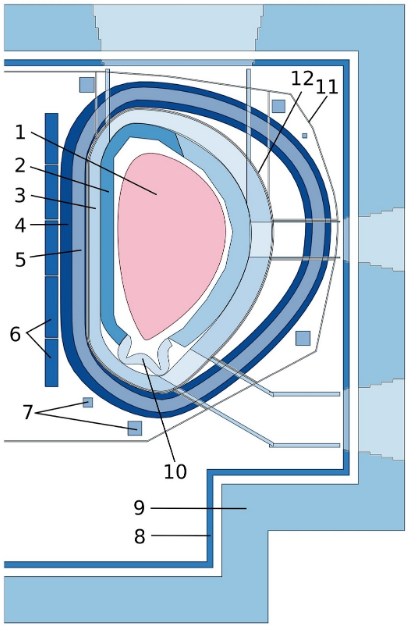
\includegraphics[width=0.48\textwidth]{fig1_tokamakdiagram.png}
  \end{center}
  \caption{Typical single-null reactor configuration as specified by BLUEPRINT \cite{Coleman2019}: 1 — plasma,
2 — breeding blankets }
\label{fig:tokamak}
\end{wrapfigure}
where T represents tritium and \isotope[7]{Li}, \isotope[6]{Li} are the more and
less frequently occurring isotopes of lithium, respectively. \isotope[6]{Li} has
the greatest tritium breeding cross-section of all tested isotopes \cite{Hernandez2018}, but due
to magnetohydrodynamic instability of liquid lithium in the reactor environment,
a variety of solid lithium compounds are preferred.

The TBR is defined as the ratio between tritium generation in the breeding
blanket per unit time and tritium fuel consumption in the reactor. The MC
neutronics simulations previously mentioned therefore must account for both the
internal plasma dynamics of the fusion reactor and the resultant interactions of
neutrons with breeding blanket materials. Neutron paths are traced through a CAD
model (e.g.~\cref{fig:tokamak}) of a reactor with modifiable geometry.

The input parameters of the computationally-expensive TBR model therefore fall
into two classes. Continuous parameters, including material thicknesses and
packing ratios, describe the geometry of a given reactor configuration. Discrete
categorical parameters further specify all relevant material sections, including
coolants, armours, and neutron multipliers. One notable exception is the
enrichment ratio, a continuous parameter denoting the presence of
\isotope[6]{Li}. Our challenge, put simply, was to produce a TBR function which
takes these same input parameters and approximates the MC TBR model with the
greatest achievable accuracy.


%---------------------------------------------------------------------

\section{Data Exploration}
\label{sec:data}
The initial step of our work is the study of the existing MC TBR model and its
behaviour. Following the examination of its features (simulation parameters), we
present efficient means of evaluating this model on large sets of points in
high-performance computing (HPC) environment, preprocessing techniques designed
to adapt collected datasets for surrogate modelling, and our attempts at feature
space reduction to achieve the lowest possible number of dimensions.


\subsection{Expensive Model Description}
\label{sec:expensive-model-description}

The MC TBR model that we understand to be the expensive function for our
surrogate modelling is fundamentally a Monte Carlo simulation based on the
OpenMC framework~\cite{ROMANO201590}. As input the software expects a set of 19~parameters, discrete and
continuous, that are fully listed in~\cref{tbl:params}. Following a brief period of
time (usually of the order of tens of seconds), during which a fixed number of
events is generated, the simulation outputs the
mean and the standard deviation of the TBR aggregated over the simulated run. The
former of these two we accept to be the output TBR value that is subject
to approximation.

\begin{table}[h]
	\centering
	{\footnotesize
		\begin{tabular}{l|llll}
		\toprule
		{} & Parameter Name & Acronym & Type & Domain\\
		\midrule
		\parbox[t]{2mm}{\multirow{12}{*}{\rotatebox[origin=c]{90}{Blanket}}}
		   & Breeder fraction\textsuperscript{\textdagger} & BBF & Continuous & $[0,1]$\\
		   & Breeder \isotope[6]{Li} enrichment fraction & BBLEF & Continuous & $[0,1]$\\
		   & Breeder material & BBM & Discrete & $\{\ce{Li2TiO3}, \ce{Li4SiO4}\}$\\
		   & Breeder packing fraction & BBPF & Continuous & $[0,1]$\\
		   & Coolant fraction\textsuperscript{\textdagger} & BCF & Continuous & $[0,1]$\\
		   & Coolant material & BCM & Discrete & $\{\ce{D2O}, \ce{H2O}, \ce{He}\}$\\
		   & Multiplier fraction\textsuperscript{\textdagger} & BMF & Continuous & $[0,1]$\\
		   & Multiplier material & BMM & Discrete & $\{\ce{Be}, \ce{Be12Ti}\}$\\
		   & Multiplier packing fraction & BMPF & Continuous & $[0,1]$\\
		   & Structural fraction\textsuperscript{\textdagger} & BSF & Continuous & $[0,1]$\\
		   & Structural material & BSM & Discrete & $\{\ce{SiC}, \text{eurofer}\}$\\
		   & Thickness & BT & Continuous & $[0,500]$\\
		\midrule
		\parbox[t]{2mm}{\multirow{7}{*}{\rotatebox[origin=c]{90}{First wall}}}
		   & Armour fraction\textsuperscript{\textdaggerdbl} & FAF & Continuous & $[0,1]$\\
		   & Coolant fraction\textsuperscript{\textdaggerdbl} & FCF & Continuous & $[0,1]$\\
		   & Coolant material & FCM & Discrete & $\{\ce{D2O}, \ce{H2O}, \ce{He}\}$\\
		   & Structural fraction\textsuperscript{\textdaggerdbl} & FSF & Continuous & $[0,1]$\\
		   & Structural material & FSM & Discrete & $\{\ce{SiC}, \text{eurofer}\}$\\
		   & Thickness & FT & Continuous & $[0,20]$\\
		\bottomrule
		\end{tabular}
	}
	\caption{Input parameters supplied to the MC TBR simulation in alphabetical
		order. Groups of fractions marked\textsuperscript{\textdagger
		\textdaggerdbl} are independently required to sum to one.}
	\label{tbl:params}
\end{table}

In our work, we often reference TBR points or samples. These are simply vectors
in the feature space generated by Cartesian product of domains of all
features---parameters from~\cref{tbl:params}.

Since most surrogate models
that we employ assume overall continuous numerical inputs, we take steps to unify our
feature interface in order to attain this property. In particular, we transform
discrete features by embedding each such feature using standard one-hot
encoding. This option is available to
us since discrete domains that generate our feature space are finite in
cardinality and relatively small in size. And while it helps us towards
unification, this step comes at the expense of increasing the dimensionality of the
feature space. This is further discussed in~\cref{sec:dimred}.


\subsection{Dataset Generation}
\label{sec:dataset-generation}

While we deliberately make no assumptions about the internal properties of the
MC TBR simulation, effectively treating it as a black box model, our means of
studying its behaviour are limited to inspection of its outputs at various
points in the feature space, and inference thereof. We thus require
sufficiently large and representative quantities of samples to ensure that
surrogates can be trained to approximate the MC TBR model.

With grid search in such a high-dimensional domain clearly intractable, we
selected uniform pseudo-random sampling\footnote{Continuous and discrete
parameters are drawn from a corresponding uniform distribution over their
domain, as defined in~\cref{tbl:params}. For reproducibility, each run uses a seed equal to its number.} to generate large amounts of feature
configurations that we consider to be independent and unbiased. For evaluation
of the expensive MC TBR model, we utilise parallelisation offered by
the HPC infrastructure available at UCL computing facilities. To this end, we
designed and implemented the Approximate TBR Evaluator---a Python software package capable of
sequential evaluation of the multi-threaded OpenMC simulation on batches of
previously generated points in the feature space.
We deployed ATE at the UCL Hypatia cluster RCIF partition, which consists of
4~homogeneous nodes, each containing 40 cores.\footnote{Hypatia RCIF nodes use
40~Intel\textsuperscript{\textregistered} Xeon\textsuperscript{\textregistered}
Gold 6148 CPUs with frequency 2.40~GHz and 376 GB RAM.} We completed three data
generation runs, which are summarised in~\cref{tbl:sampling-runs}.

\begin{table}[h]
	\sisetup{round-mode=places,round-precision=2}
	\centering
	{\footnotesize
		\begin{tabular}{rlllll}
		\toprule
		\#	& Samples & Batch division & $t_{\text{run}} $ 
			& $\overline{t}_{\text{eval.}}$ [\si{\second}] & Description \\
		\midrule
		0 & \num{100000} & $\num{100}\times\num{1000}$ & 2~days, 23~h 
		  & $\num{7.877122043981347} \pm \num{2.749485948560108}$ &
		Testing run using old MC TBR version.\\
		1 & \num{500000} & $\num{500}\times\num{1000}$ & 13~days, 20~h
		  & $\num{7.777049573054314} \pm \num{2.8103592103930337}$ &
		Fully uniform sampling in the entire domain.\\
		2 & \num{400000} & $\num{400}\times\num{1000}$ & 10~days 
		  & $\num{7.944379778103232} \pm \num{2.601428571503671}$ &
		Mixed sampling, discrete features fixed.\\
		\bottomrule
		\end{tabular}
	}
	\caption{Parameters of sampling runs. Here, $t_{\text{run}}$ denotes the total run
		time (including waiting in the processing queue), and
		$\overline{t}_{\text{eval.}}$ is the mean evaluation time of MC TBR (per single
		sampled point).}
	\label{tbl:sampling-runs}
\end{table}

Skipping run zero, which was performed using an older, fundamentally different
version of the MC TBR software, and was thus treated as a technical
proof-of-concept, we generated a total of~\num{900000} samples in two runs.
While the first run featured fully uniform sampling of the unrestricted feature
space, the second run used a more elaborate strategy. Interested in further study
of relationships between discrete and continuous features, we selected four
assignments of discrete features (listed in~\cref{tbl:slices}) and fixed them
for all points, effectively slicing the feature space into four corresponding
subspaces. In order to achieve comparability, all such \textit{slices} use the
same samples for the values of continuous features.

\begin{table}[h]
	\centering
	{\footnotesize
		\begin{tabular}{rllllll}
		\toprule
		{} & \multicolumn{6}{c}{Discrete feature assignment}\\
		\cmidrule(lr){2-7}
		Batches & BBM & BCM & BMM & BSM & FCM & FSM \\
		\midrule
		0-99 & \ce{Li4SiO4} & \ce{H2O} & \ce{Be12Ti} & eurofer & \ce{H2O} & eurofer\\
		100-199 & \ce{Li4SiO4} & \ce{He} & \ce{Be12Ti} & eurofer & \ce{H2O} & eurofer\\
		200-299 & \ce{Li4SiO4} & \ce{H2O} & \ce{Be12Ti} & eurofer & \ce{He} & eurofer\\
		300-399 & \ce{Li4SiO4} & \ce{He} & \ce{Be12Ti} & eurofer & \ce{He} & eurofer\\
		\bottomrule
		\end{tabular}
	}
	\caption{Selected discrete feature assignments corresponding to slices in run~2.}
	\label{tbl:slices}
\end{table}

Since some surrogate modelling methods applied in this work are not scale-invariant or
perform suboptimally with arbitrarily scaled inputs, all obtained TBR~samples
(features and TBR~values) were standardised prior to further use. In this
commonly used statistical procedure, features and regression outputs are
independently scaled and offset to attain zero mean and unit variance.



\subsection{Dimensionality Reduction}
\label{sec:dimred}

% TODO: here maybe mention desirable effects of dim. red. (e.g. speedup,
% simplification of the problem, better convergence...)

Model training over high-dimensional parameter spaces (illustrated
in~\cref{fig:tbr-vs-features}) may be improved in many
aspects by carefully reducing the number of variables used to describe the
space. For many applications, feature selection strategies succeed in
identifying a sufficiently representative subset of the original input
variables; however, all given variables were assumed to be physically relevant
to the MC TBR model. Feature extraction methods, on the other hand, aim to
identify a transformation of the parameter space which decreases dimensionality; even if no individual parameter is separable from the space, some linear combinations of parameters or nonlinear functions of parameters may be.

\begin{figure}[h]
	\centering
	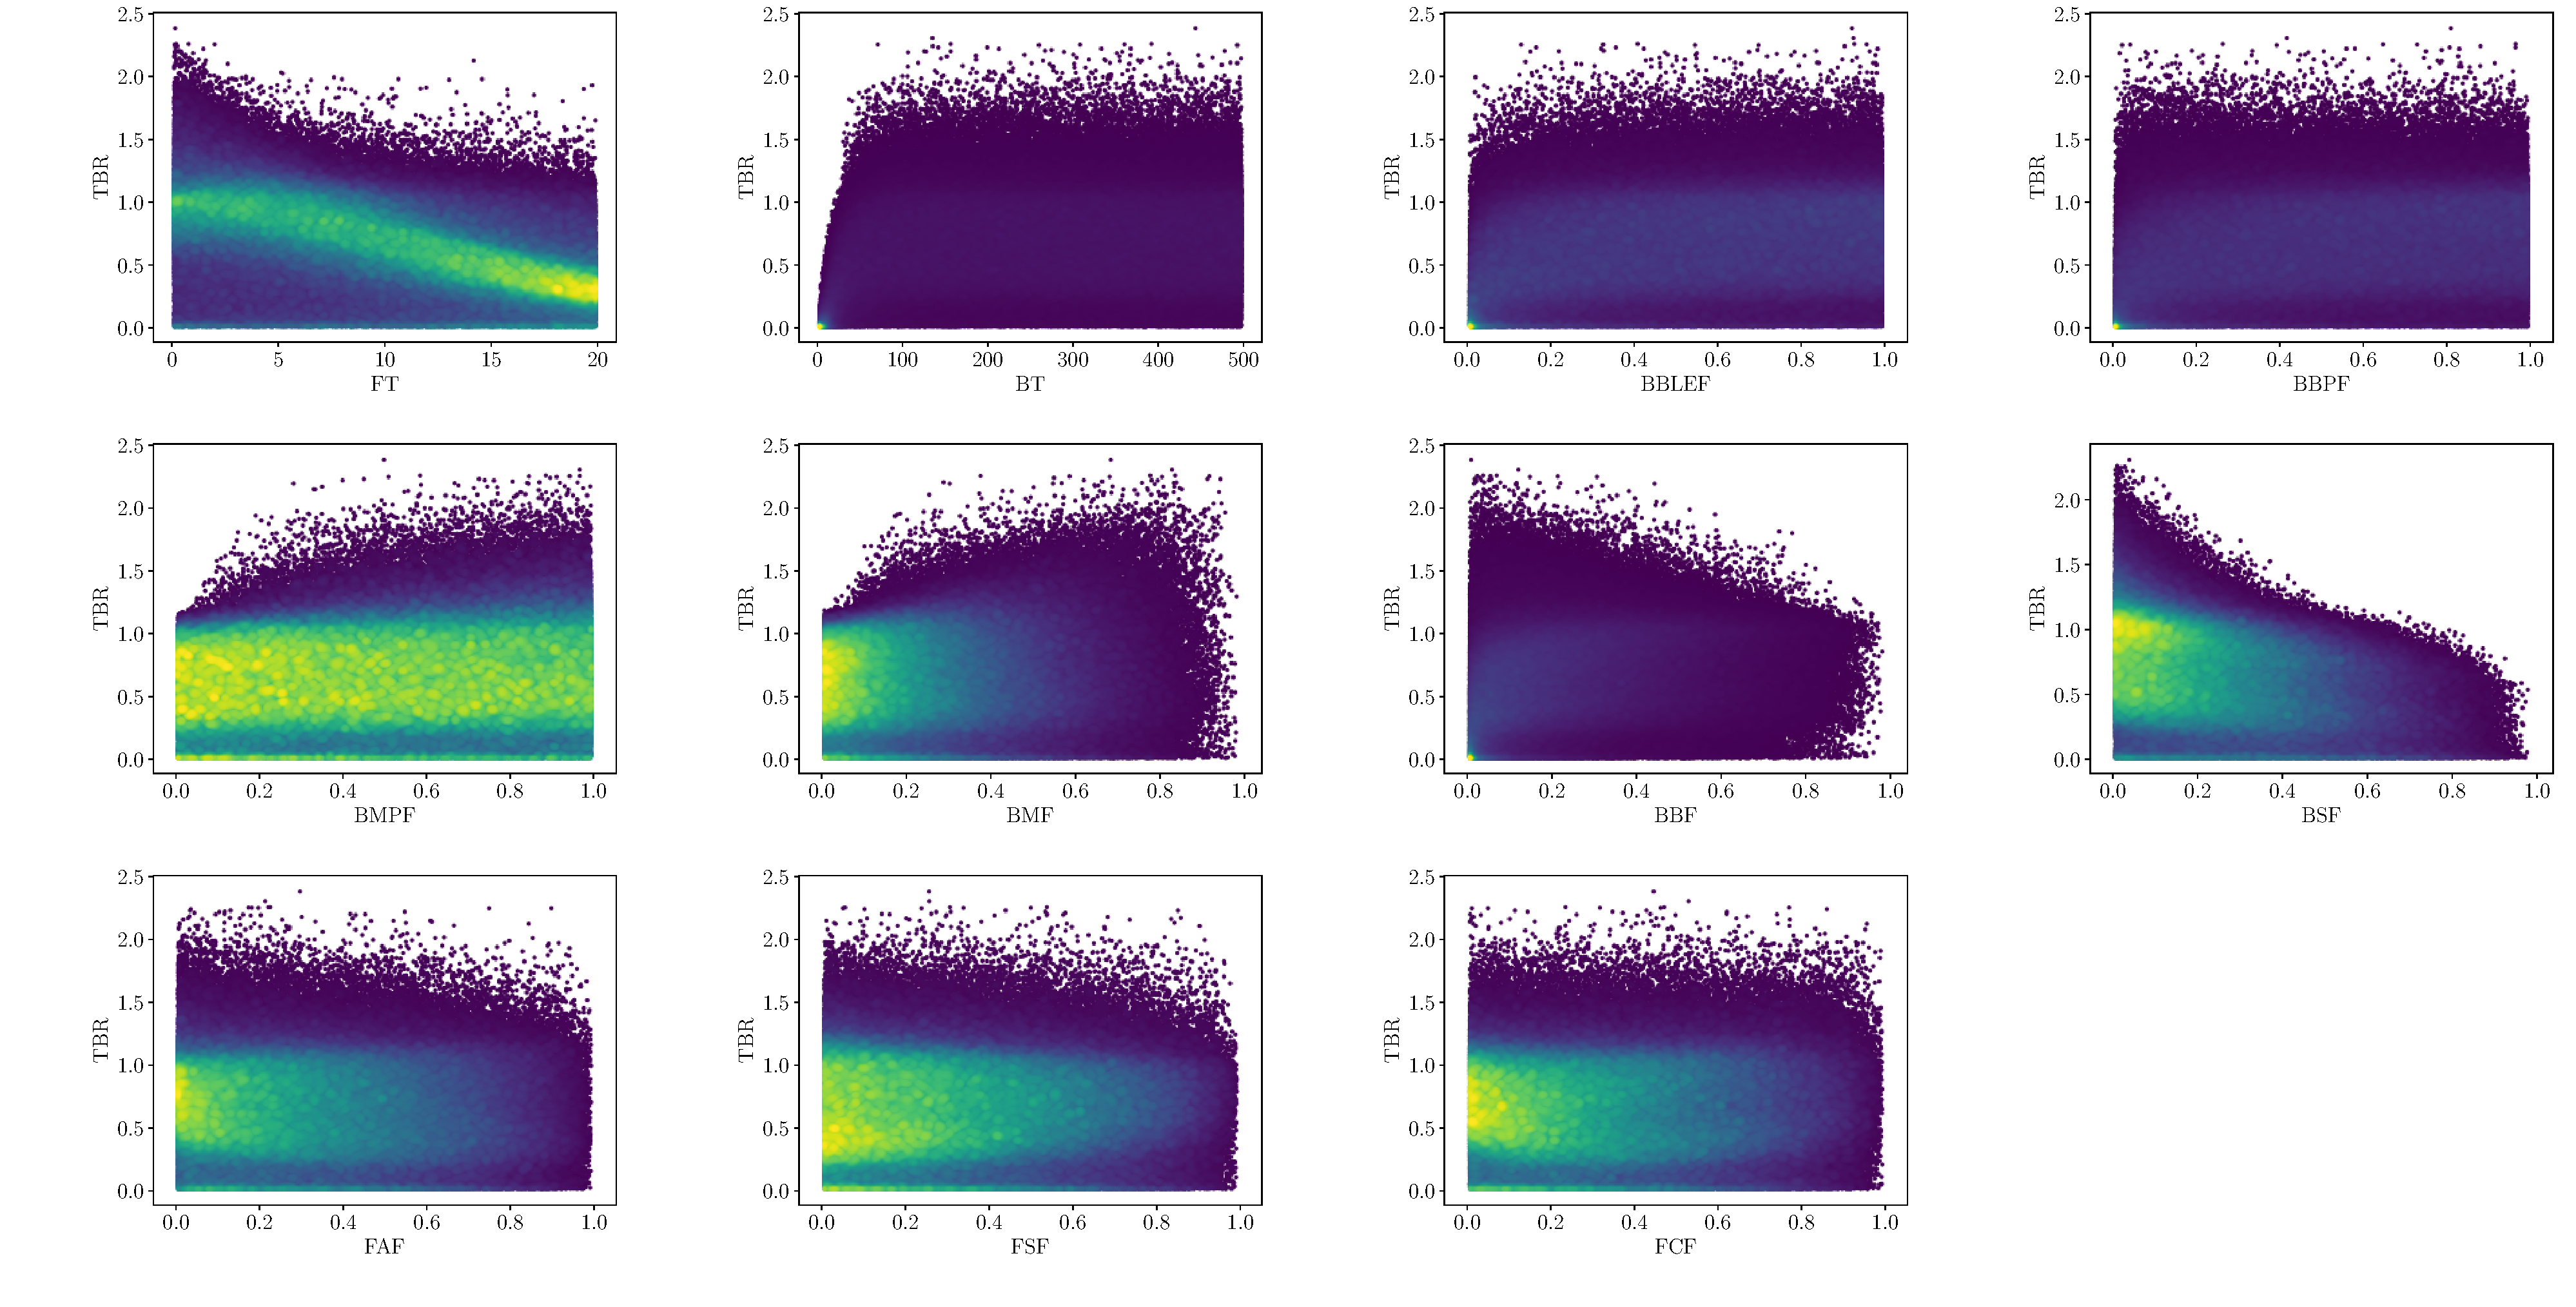
\includegraphics[width=\linewidth]{run1_500k_tbr_vs_feat}
	\caption{Marginalised dependence of TBR on the choice of continuous
	features in \num{500000}~points collected in run~1. Points are coloured by density.}
  \label{fig:tbr-vs-features}
\end{figure}


\subsubsection{Principal Component Analysis}

To pursue linear feature extraction, principal component analysis (PCA)
\cite{Jolliffe2016} was performed via SciKit Learn~\cite{scikit-learn} on a set
of \num{300000} uniform samples of the MC TBR model. % TODO:which run? batch range?

\Cref{fig:pca} shows the resultant cumulative variance of the 11 principal components. The similar share of variance among all features
reveals irreducibility of the TBR model by linear methods.

\begin{figure}[h]
	\centering
	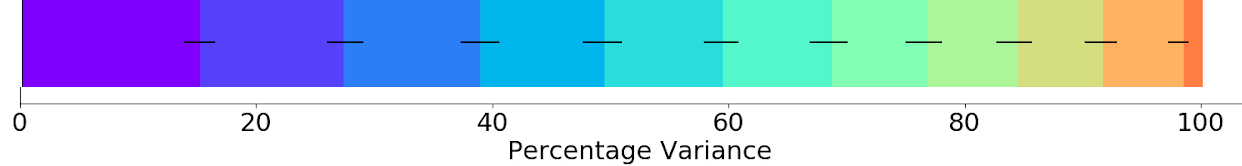
\includegraphics[width=0.6\linewidth]{fig2_pca.jpg}
	\caption{Cumulative variance for optimal features identified by PCA}
	\label{fig:pca}
\end{figure}

\begin{wrapfigure}[30]{r}{0.5\textwidth}
	\centering
	\hspace*{-.3\columnsep}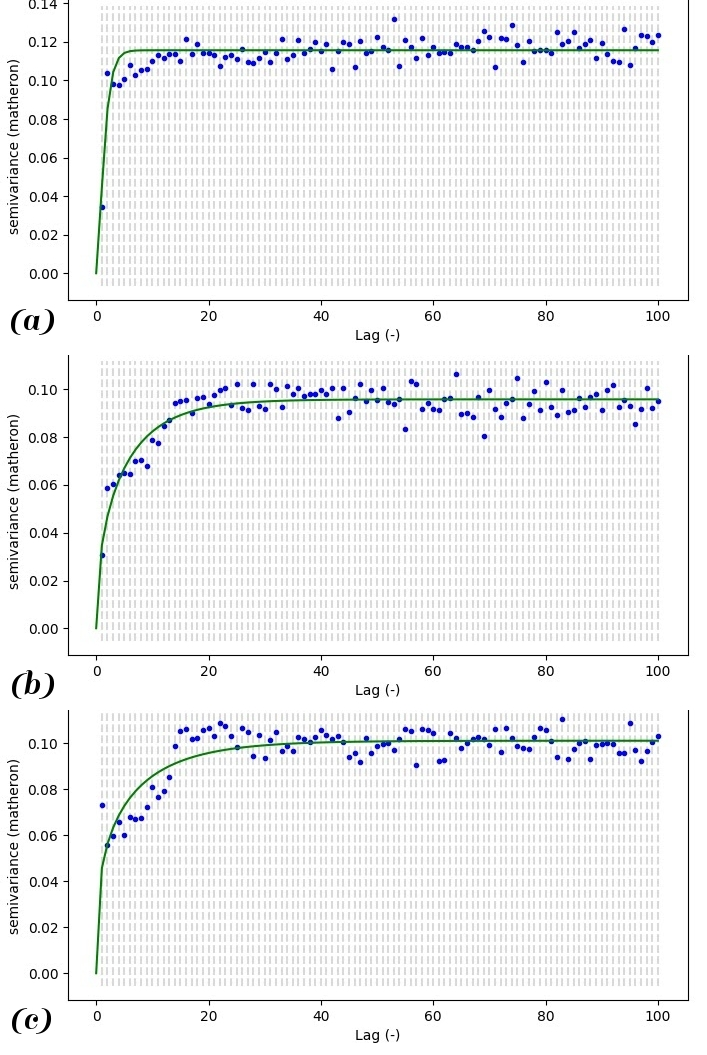
\includegraphics[width=0.58\textwidth]{fig3_allvar.jpg}
	\caption{Semivariograms for MC TBR data with coolant materials: (a) \ce{He},
	(b) \ce{H2O}, (c) \ce{D2O}}
	\label{fig:var}
\end{wrapfigure}

\subsubsection{Variogram Computations}

Kriging is a geostatistical surrogate modelling technique which relies on
correlation functions over distance (lag) in the feature space \cite{Bouhlel2018}. Although kriging performed poorly for our use case due to high dimensionality, these correlation measures gave insight into similarities between discrete-parameter slices of the data.

\Cref{fig:var} shows the Matheron semivariance \cite{Matheron1963} for three discrete slices with coolant material varied, but all other discrete parameters fixed. Fits \cite{KrigingFig} to the Matérn covariance model confirmed numerically that the coolant material is the discrete parameter with the greatest distinguishability in the MC TBR model. 


\subsubsection{Autoencoders}

Autoencoders~\cite{SCHMIDHUBER201585} are a family of approaches to
dimensionality reduction driven by artificial neural
networks (ANNs). Faced with a broad selection of alternatives, we opted for a
conventional autoencoder architecture with a single hidden layer. While it
follows that the input and output layers of such
network are sized to accommodate the analysed dataset, the
hidden layer, also called \textit{the bottleneck}, allows for variable number of
neurons that represent a smaller subspace. By scanning
over a range of bottleneck widths and investigating relative changes in the
validation loss, we assess the potential for dimensional reduction.

\begin{wrapfigure}[15]{l}{0.25\textwidth}
	\centering
	{\footnotesize \incfigscale{0.8}{autoencoder}}
	\caption{Autoencoder with input width~$W_0$ and bottleneck width~$W_1$.
	Here, $\text{Dense}(N)$ denotes a fully-connected layer of $N$ neurons.}
	\label{fig:autoencoder}
\end{wrapfigure}

In particular, we consider two equally-sized sets\footnote{Each set contained
\num{100000}~samples from batches 0-99 of the corresponding runs.} of samples:
(i)~a subset of data obtained
from run~1 and (ii)~a subset of a single slice obtained from run~2. Our
expectation was that while the former case would provide meaningful insights into
correlations within the feature space, the latter would validate our
autoencoder implementation by analysing a set of points that are trivially
reducible in dimensionality due to a number of fixed discrete features.

\begin{wrapfigure}[22]{r}{0.4\textwidth}
	\centering
	\vspace{-4ex}

	\begin{subfigure}[b]{\linewidth}
		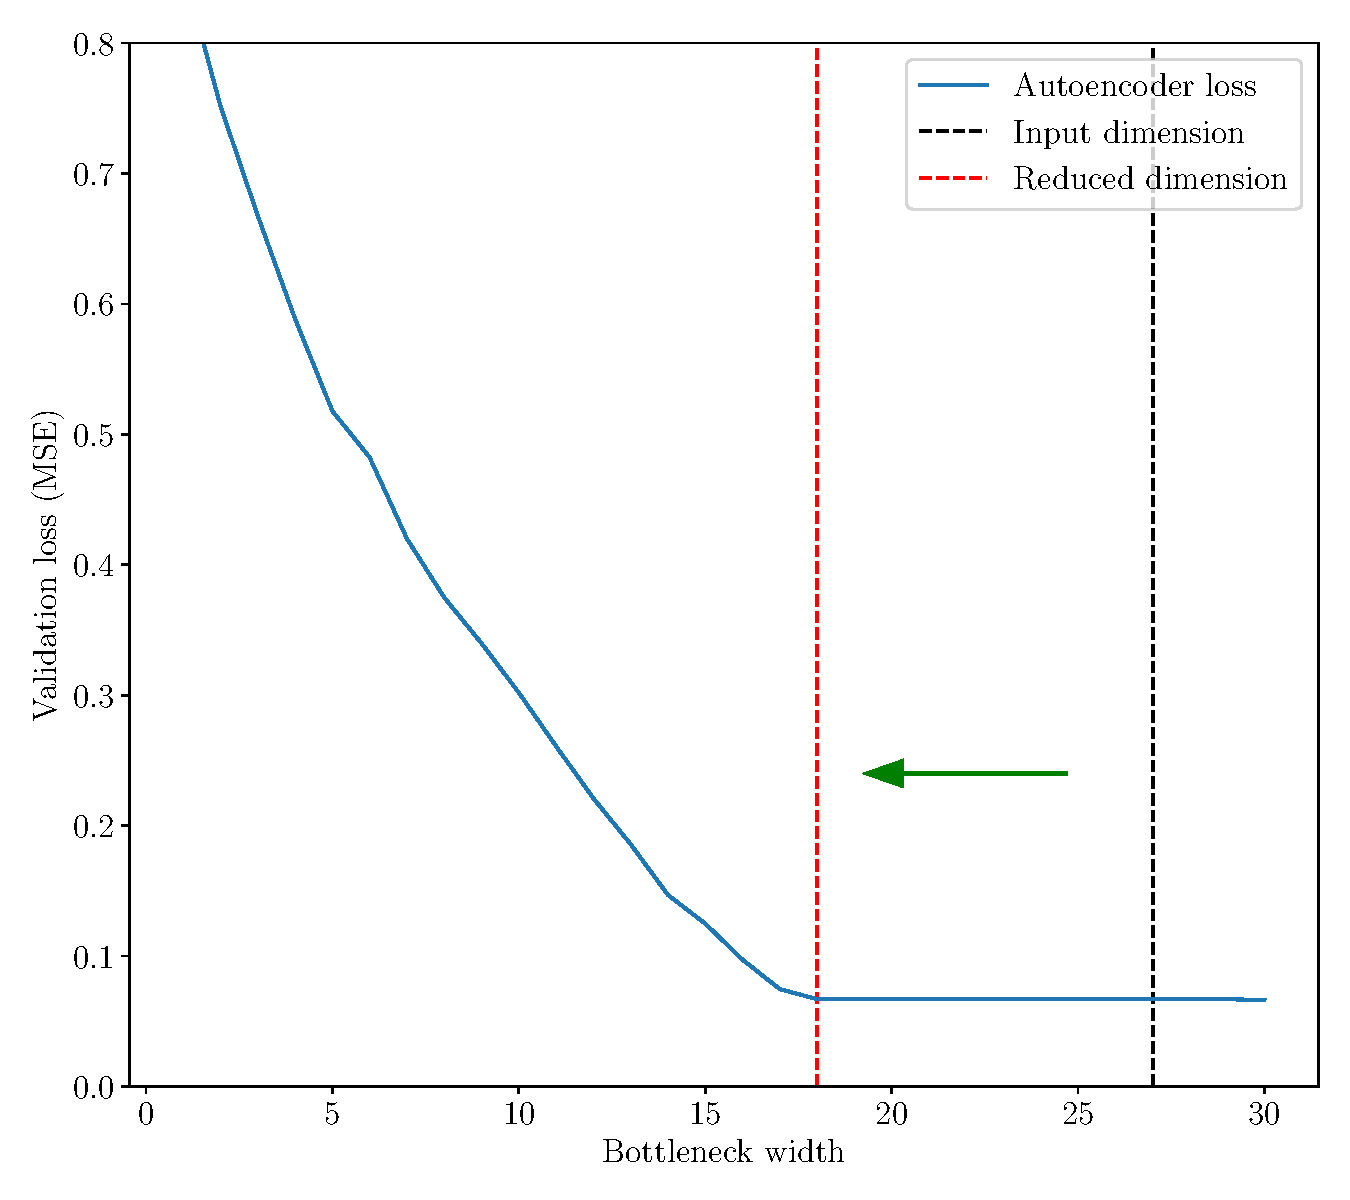
\includegraphics[width=\linewidth,trim={0 48px 0 0},clip]{ae_mixed}
	\end{subfigure}

	\vspace{-0.2ex}

	\begin{subfigure}[b]{\linewidth}
		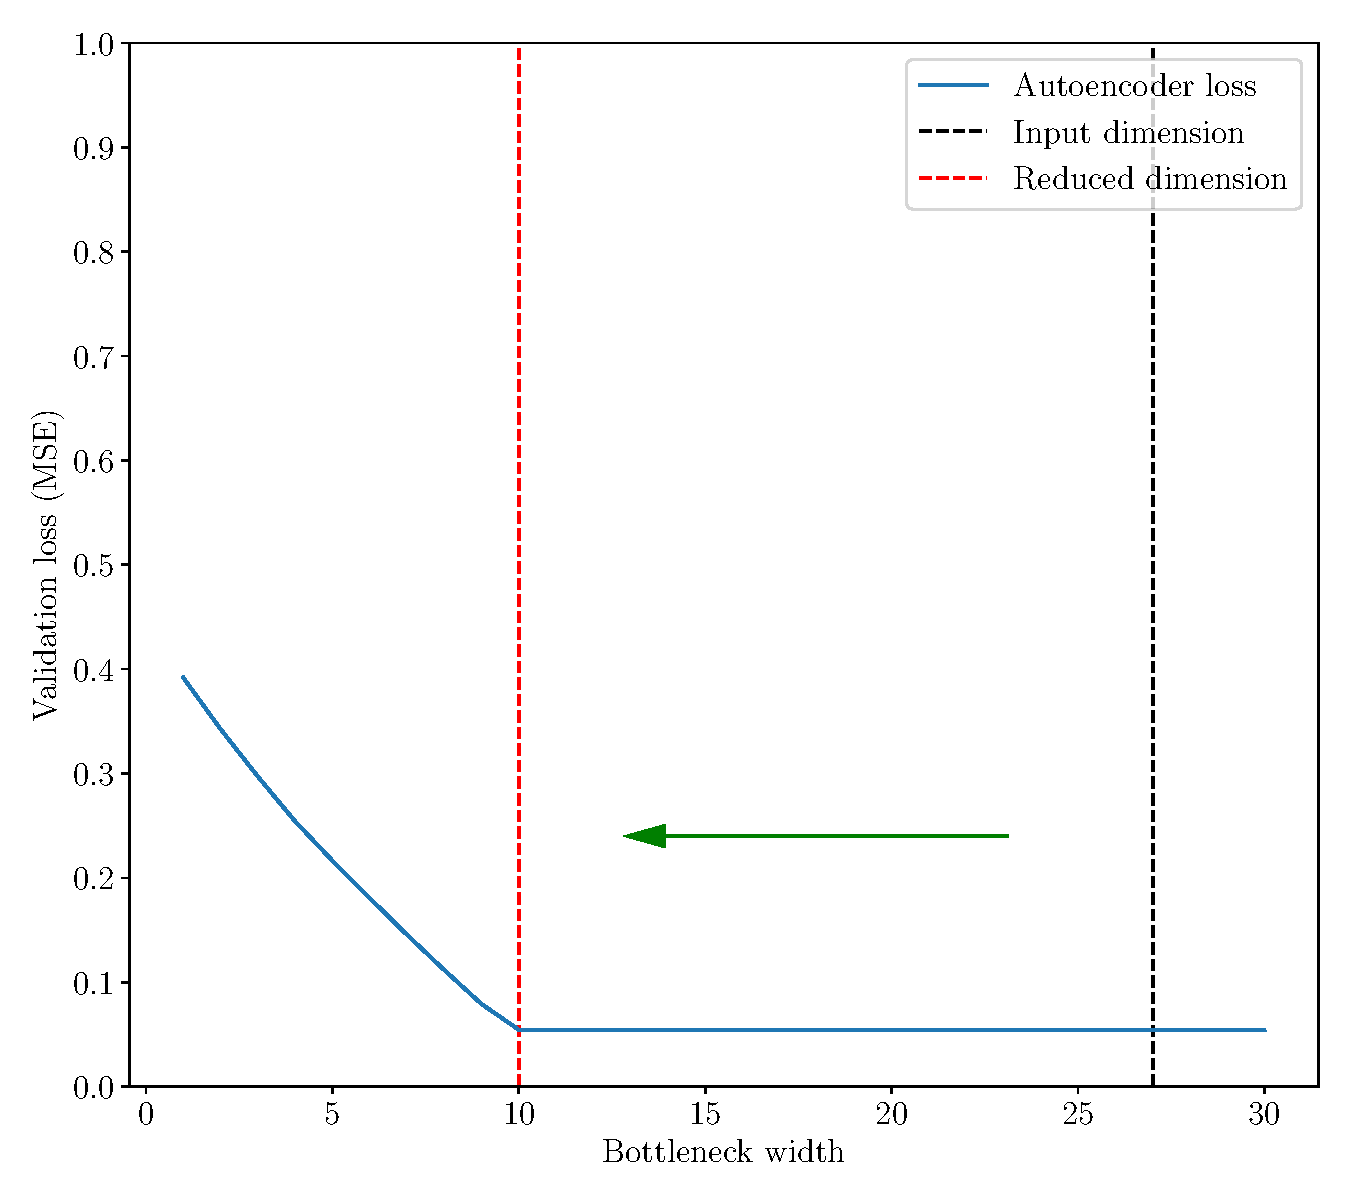
\includegraphics[width=\linewidth]{ae_single_slice}
	\end{subfigure}

	\caption{Autoencoder loss scan on the full feature space (top) and a single slice
		(bottom). Dimensional reduction is indicated by a green arrow.}
	\label{fig:autoencoder-loss}
\end{wrapfigure}

The results of both experiments are shown in~\cref{fig:autoencoder-loss}.
Consistent with our motivation, in each plot we can clearly identify a constant
plateau of low error in the region of large dimensionality followed by a point,
from which a steep increase is observed.
We consider this \textit{critical point} to mark the largest viable
dimensional reduction without significant information loss.
With this approach we find that the autoencoder was able to reduce the
datasets into a subspace of 18~dimensions in the first case and 10~dimensions in
the second case.

Confirming our expectation that in the latter, trivial case the
autoencoder should achieve greater dimensional reduction, we are inclined to
believe that our implementation is indeed operating as intended. However, we
must also conclude that in both examined cases this method failed to produce a
reduction that would be superior to a naïve approach.\footnote{In both tested cases we
	can trivially eliminate 7~dimensions due to overdetermined one-hot-encoded
	features and 2~dimensions due to sum-to-one constraints. Furthermore, in the
	single slice case we may omit 7~additional dimensions due to artificially fixed
features.} This is consistent with previous results obtained by PCA and kriging.


% TODO: Question: is it accurate to say this represents nonlinear feature extraction? re my intro paragraph


%---------------------------------------------------------------------

\section{Methodology}
\label{sec:methodology}
Assuming that input has been appropriately treated to eliminate redundant
features, we may turn to characterise proposed surrogate models and the criteria
used for their evaluation. The task all presented surrogates strive to solve can be
formulated using the language of conventional regression problems. In the scope
of this work, we explore various possible choices available to us in the
scheme of supervised and unsupervised learning.

Labeling the expensive Monte Carlo simulation $f(x)$, a surrogate is a mapping
$\hat{f}(x)$ that yields similar images as $f(x)$. In other words, $f(x)$ and
$\hat{f}(x)$ minimise a selected similarity metric. Furthermore, in order to
be considered \textit{viable}, surrogates are required to achieve expected evaluation time
that does not exceed the expected evaluation time of $f(x)$.

In the supervised learning setting, we first gather a sufficiently large
training set of samples $\mathcal{T}=\left\{\left( x^{(i)},f\left(x^{(i)}\right) \right)\right\}_{i=1}^N$
to describe the behaviour of $f(x)$ across its domain.
Depending on specific model class and appropriate choice of its
hyperparameters, surrogate models $\hat{f}(x)$ are trained to minimise
empirical risk with respect to $\mathcal{T}$ and a model-specific
loss function $\mathcal{L}$, where empirical risk is defined as

\begin{align}
	R_{\text{emp.}}(\hat{f}\mid\mathcal{T},\mathcal{L})
	=\frac{1}{N}\sum_{i=1}^N
	\mathcal{L}\left(\hat{f}(x^{(i)}),f(x^{(i)})\right).
\end{align}

The unsupervised setting can be viewed as an extension of this method.
Rather than fixing the training set $\mathcal{T}$ for the entire duration of
training, multiple sets $\{\mathcal{T}_k\}_{k=0}^K$ are used, such that
$\mathcal{T}_{k-1}\subset\mathcal{T}_k$ for all $k>1$. The first set
$\mathcal{T}_0$ is initialised randomly to provide a \textit{burn-in}, and is
repeatedly extended in epochs, whereby each epoch trains a new surrogate on
$\mathcal{T}_k$ using the supervised learning procedure, evaluates its
performance, and forms a new set $\mathcal{T}_{k+1}$ by adding more samples to
$\mathcal{T}_k$. This permits the learning algorithm to condition the selection
of new samples by the results of evaluation in order to focus on improvement of
surrogate performance in complex regions within the domain.


\subsection{Metrics}
\label{sec:metrics}

Aiming to provide objective comparison of a diverse set of surrogate model
classes, we define a multitude of metrics to be tracked during experiments.
Following the motivation of this work, two desirable properties of surrogates
arise: (i) their capability to approximate the expensive
model well and (ii) their time of evaluation. An ideal surrogate would maximise
the former while minimising the latter.

\Cref{tbl:metrics} provides exhaustive listing and description of metrics recorded
in the experiments. For regression performance analysis, we include a selection
of absolute metrics to assess the approximation capability of surrogates, and set
practical bounds on the expected accuracy of their predictions. In addition, we also track
relative measures that are better-suited for model comparison between works as
they maintain invariance with respect to the selected domain and image space.
For analysis of evaluation time, surrogates are assessed in terms of wall time
elapsed during training and predicition. This closely models the practical use
case, in which they are trained and used as drop-in replacements for the
expensive model. Since training set sizes remain to be determined, all times are
reported per a single sample. Even though some surrogates support acceleration
by means of parallelisation, measures were taken to ensure sequential
processing of samples to achieve comparability between considered models.

\begin{table}[h]
	\centering
	\begin{tabular}{llrl}
	\toprule
	Regression performance metrics	& Mathematical formulation / description &
	\multicolumn{2}{c}{Ideal value} \\
	\midrule
	Mean absolute error (MAE)	& $\sum_{i=1}^N |y^{(i)}-\hat{y}^{(i)}|/N$ & 0
								& [TBR] \\
	Standard error of regression $S$	& $\text{StdDev}_{i=1}^N\left\{ |y^{(i)} -
	\hat{y}^{(i)}| \right\} $	 & 0 & [TBR] \\
	Coefficient of determination $R^2$	& $1-\sum_{i=1}^N \left(y^{(i)}-\hat{y}^{(i)} \right)^2 /
	\sum_{i=1}^N \left( y^{(i)}-\overline{y} \right)^2 $ & 1 & [rel.] \\
	Adjusted $R^2$	& $1-(1-R^2)(N-1)/(N-P-1)$	& 1 & [rel.] \\
	\midrule
	Evaluation time metrics	& {} & {} & {} \\
	\midrule
	Mean training time $\overline{t}_{\text{trn.}}$	& $(\text{wall training time of
	$\hat{f}(x)$})/N_0$ 	& 0 & [ms] \\
	Mean prediction time $\overline{t}_{\text{pred.}}$	& $(\text{wall prediction time of
	$\hat{f}(x)$})/N$	& 0 & [ms] \\
	Relative speedup	& $(\text{wall evaluation time of $f(x)$}) /
	(N\overline{t}_{\text{pred.}})$	&
	$\to\infty$ & [rel.] \\
	\bottomrule
	\end{tabular}
	\caption{Metrics recorded in supervised learning experiments. In
	formulations, we work with training set of size $N_0$ and testing set of
size $N$, TBR values $y^{(i)}=f(x^{(i)})$ and $\hat{y}^{(i)}=\hat{f}(x^{(i)})$
denote images of the $i$th testing sample in the expensive model and the surrogate
respectively. Furthermore, the mean $\overline{y}=\sum_{i=1}^N y^{(i)}/N$ and $P$ is the
number of input features.}
	\label{tbl:metrics}
\end{table}

To prevent undesirable bias in results due to training set selection, all metrics
collected in the scheme of $k$-fold cross-validation with a standard choice of
$k=5$. Herein, a sample set is subdivided into 5 disjoint folds which are
repeatedly interpreted as training and testing sets, maintaining a constant
ratio of samples between the two. In each such interpretation experiments are
repeated, and the overall value of each metric of interest is reported as the
mean across all folds.


\subsection{Supervised Learning Experiments}
\label{sec:supervised}

\subsubsection{Considered Surrogates}

\begin{table}[h]
	\centering
	\begin{tabular}{llll}
	\toprule
	Surrogate & Acronym & Implementation & Hyperparameters \\
	\midrule
	Support vector machines	& SVM & SciKit Learn & TODO \\
	Gradient boosted trees	& GBT & SciKit Learn & TODO \\
	Extremely random trees	& ERT & SciKit Learn & TODO \\
	AdaBoost	& AB & SciKit Learn & TODO \\
	Gaussian process regression	& GPR & SciKit Learn & TODO \\
	$k$ nearest neighbours	& KNN & SciKit Learn & TODO \\
	Neural networks	& NN & Keras (TensorFlow) & TODO \\
	Inverse distance weighing & IDW & SMT & TODO \\
	Radial basis functions & RBF & SMT & TODO \\
	Stochastic gradient descent & SGD & SciKit Learn & TODO \\
	Ridge regression & RR & SciKit Learn & TODO \\
	Kriging & KRG & SMT & TODO \\
	\bottomrule
	\end{tabular}
	\caption{TODO}
	\label{tbl:surrogates}
\end{table}

TODO: describe classes of surrogates

TODO: reference implementations and original papers

TODO: define NN architectures


\subsubsection{Experiments}

TODO: single slice hyperparameter optimisation

TODO: multislice (mixed) hyperparameter optimisation

TODO: retraining for scaling benchmark

TODO: retraining on large set

\subsection{Adaptive Sampling}
\label{sec:adaptive}


%---------------------------------------------------------------------

\section{Results}
\label{sec:results}
Having outlined a variety of models and metrics tracked for the
purposes of their objective comparison, we proceed to present and discuss our
results in the next sections.


\subsection{Results of Decoupled Sampling}
\label{sec:modelres}

We begin by comparing a diverse set of surrogate families that we proposed
to evaluate on previously collected samples of the expensive MC TBR model.
Through the four experimental cases described
in~\cref{sec:experiment-methodology}, we aim to study properties of the
considered models in terms of regression performance, training and prediction
time.

\subsubsection{Hyperparameter Tuning}

The first two experiments perform Bayesian optimisation to maximise~$R^2$ in
a cross-validation setting as a function of model hyperparameters. While in the
first experiment we limit training and test sets to the scope of four selected
slices of the feature space, in the second experiment we lift this restriction.

The results displayed in~\cref{fig:exp1-time-vs-reg} indicate that in the first
experiment, GBTs clearly appear to be the most accurate as
well as the fastest surrogate family in terms of mean prediction time. Following
that, we note that ERTs, SVMs and ANNs also achieved satisfactory results with respect to both examined metrics.
While the remainder of tested surrogate families does not exhibit problems in
complexity, its regression performance falls below average.

\begin{figure}[h]
	\centering
	\begin{subfigure}[b]{0.333\textwidth}
		\centering
		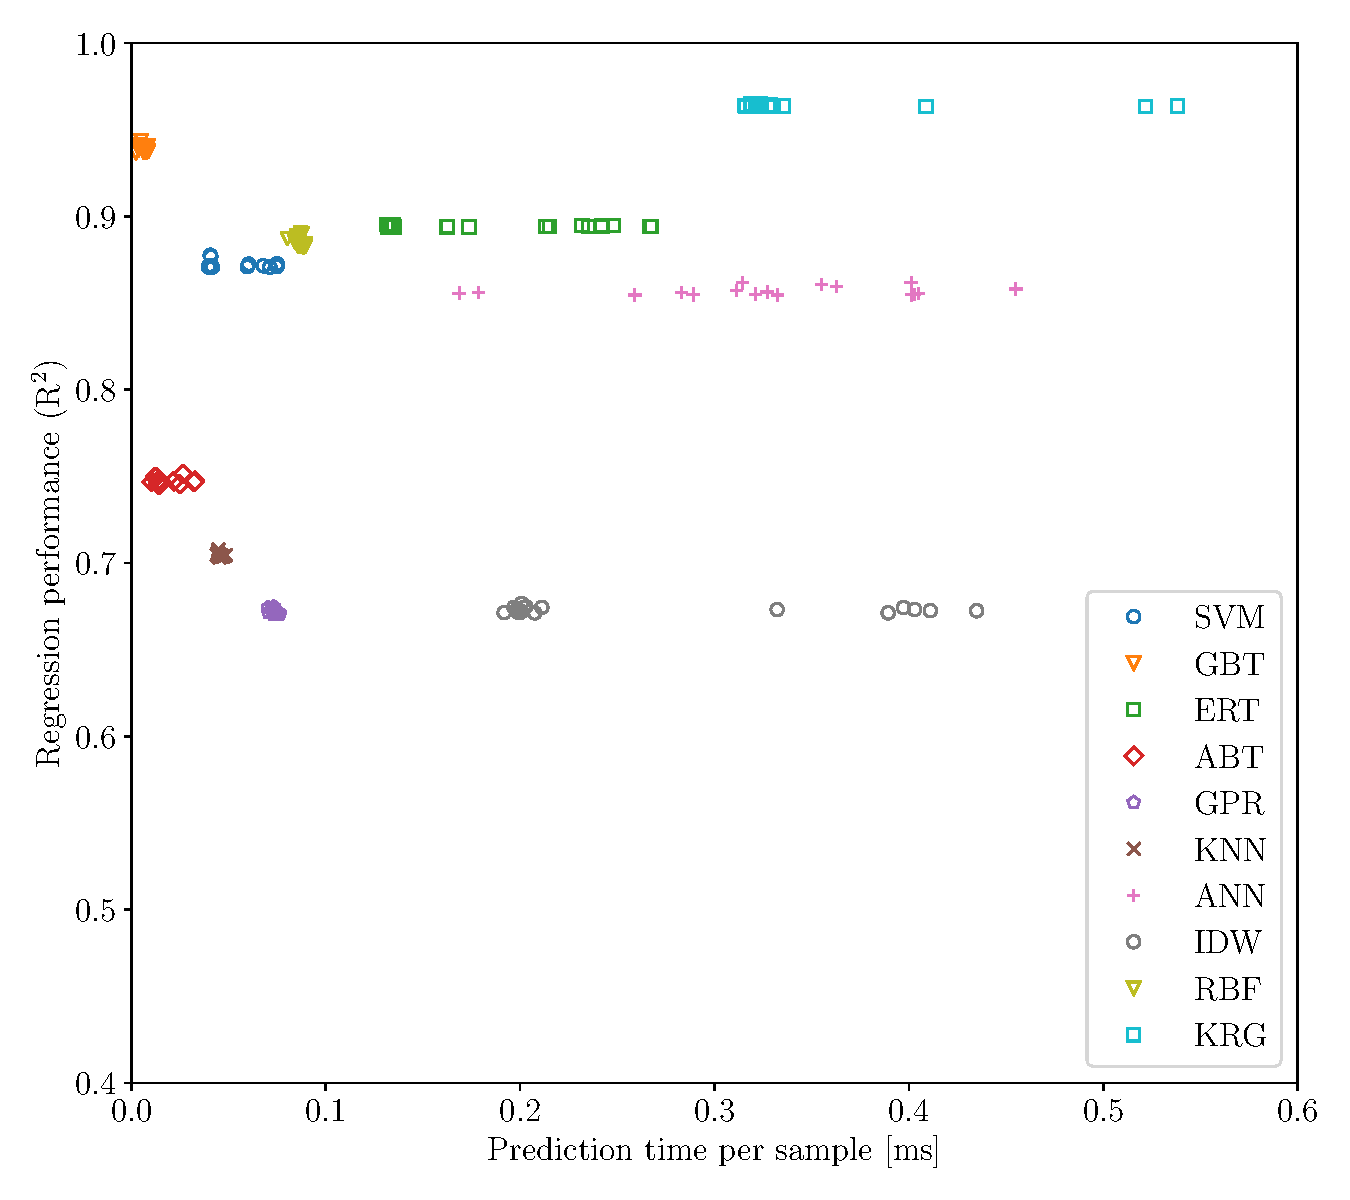
\includegraphics[width=\linewidth]{exp1_slice0}
		\caption{Run 2, batches 0-2}
	\end{subfigure}\hfill%
	\begin{subfigure}[b]{0.333\textwidth}
		\centering
		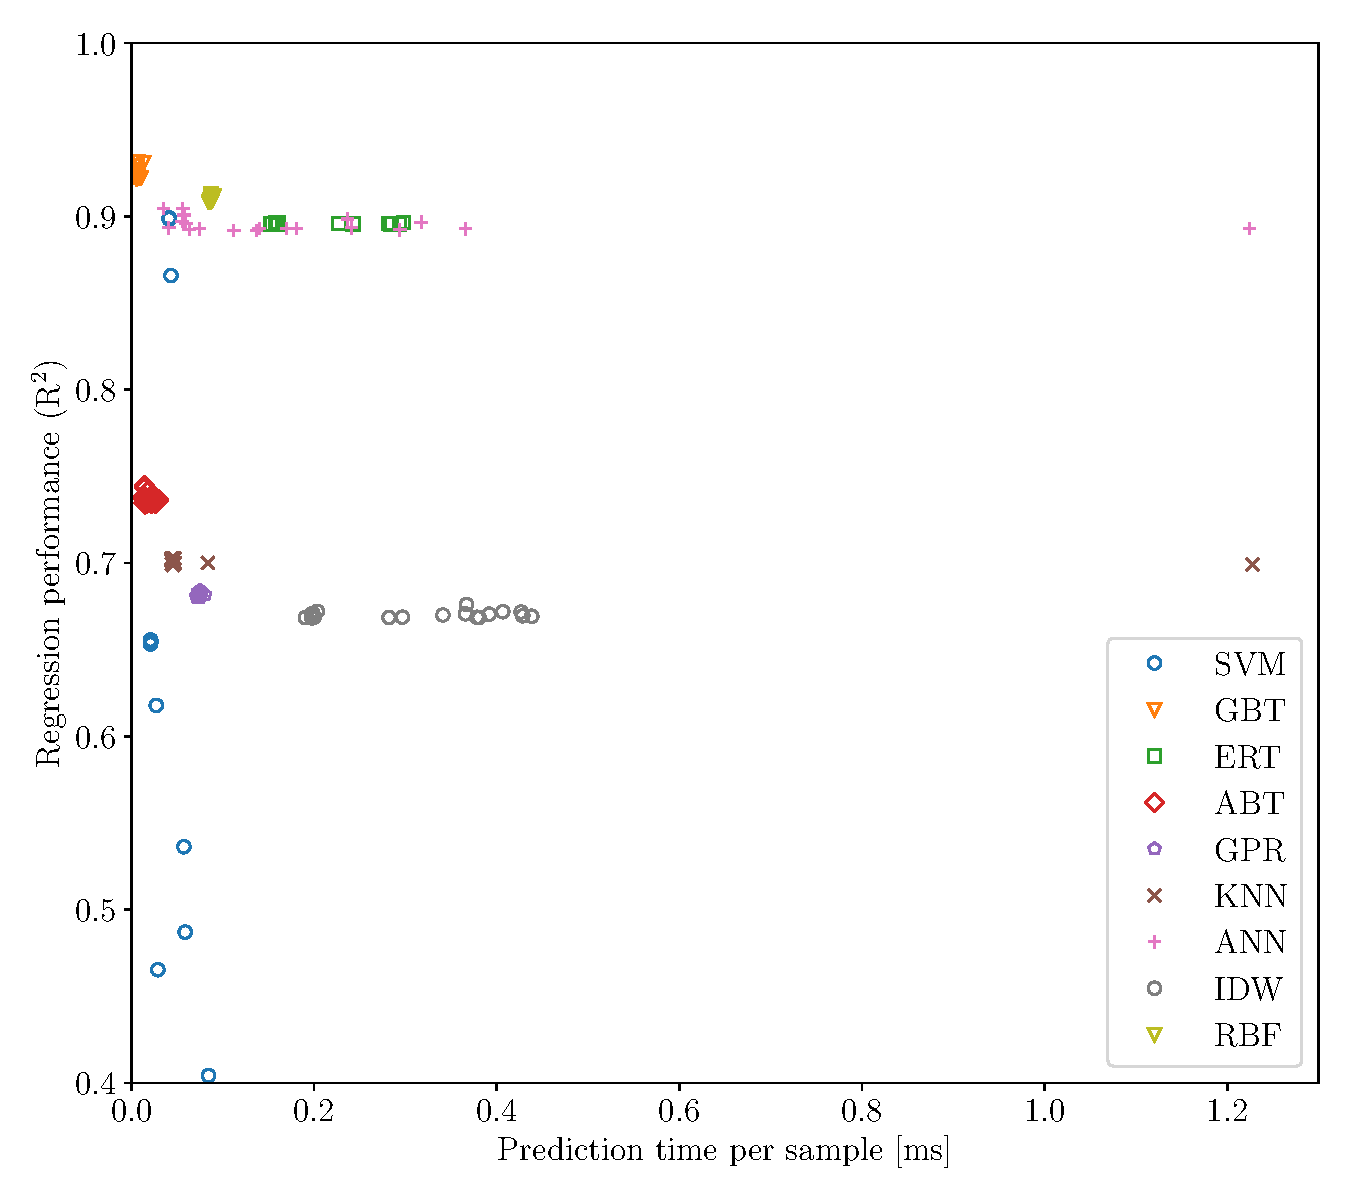
\includegraphics[width=\linewidth]{exp1_slice1}
		\caption{Run 2, batches 100-102}
	\end{subfigure}\hfill%
	\begin{subfigure}[b]{0.333\textwidth}
		\centering
		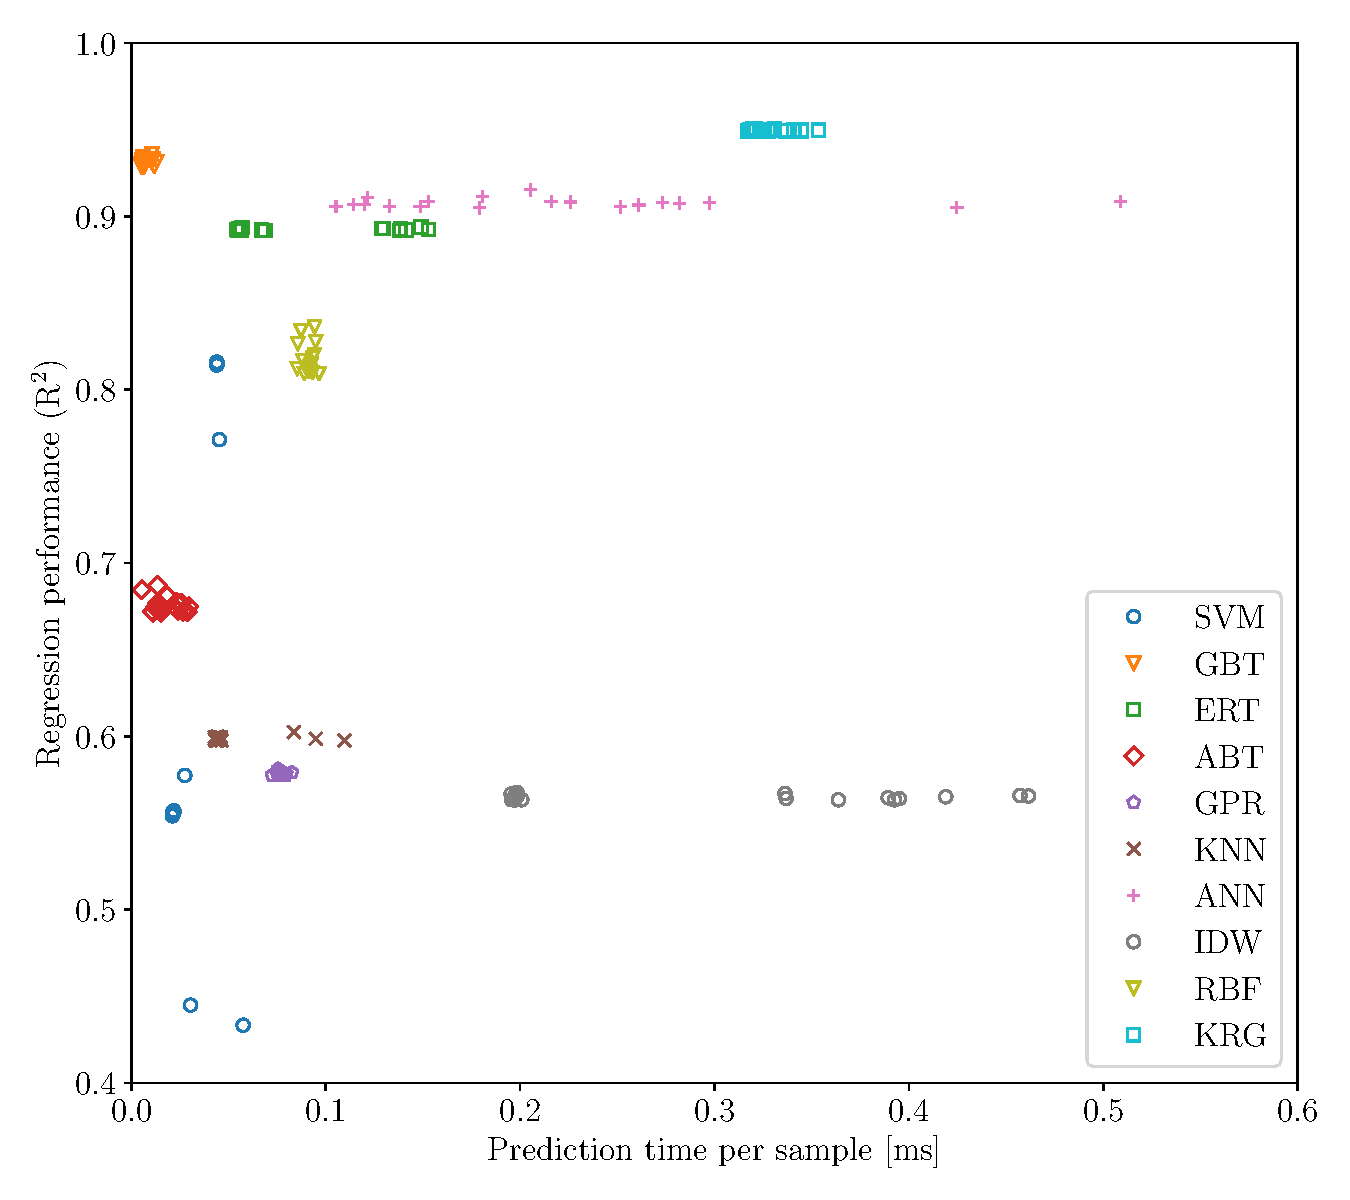
\includegraphics[width=\linewidth]{exp1_slice2}
		\caption{Run 2, batches 200-202}
	\end{subfigure}
	\caption{20~best-performing surrogates per each considered family, plotted in
		terms of complexity (as $\overline{t}_{\text{pred.}}$) and regression
		performance (as~$R^2$) on selected slices of run~2, evaluated in
	experiment~1. Here, batches refer to subsets of training and test datasets that
	may be matched to slices using~\cref{tbl:slices}.}
	\label{fig:exp1-time-vs-reg}
\end{figure}

The results of the second experiment, shown in~\cref{fig:exp2-time-vs-reg},
seem to confirm our expectations. Compared to the previous case, we observe
that many surrogate families consistently achieved worse regression
performance and prediction times in a more complex, unrestricted domain. The least
affected models appear to be GBTs, ANNs and ERTs, which are known to be capable of capturing relationships
involving mixed feature types that were deliberately withheld in the first
experiment. With only negligible differences, the first two of these families
appear to be tied for the best performance as well as the shortest prediction
time. We observe that ERTs trees and RBFs also
demonstrated satisfactory results, outperforming the remaining surrogates in
terms of regression performance, and in some cases also in prediction time.

\begin{wrapfigure}[10]{r}{0.333\textwidth}
	\centering
	\vspace{-2ex}
	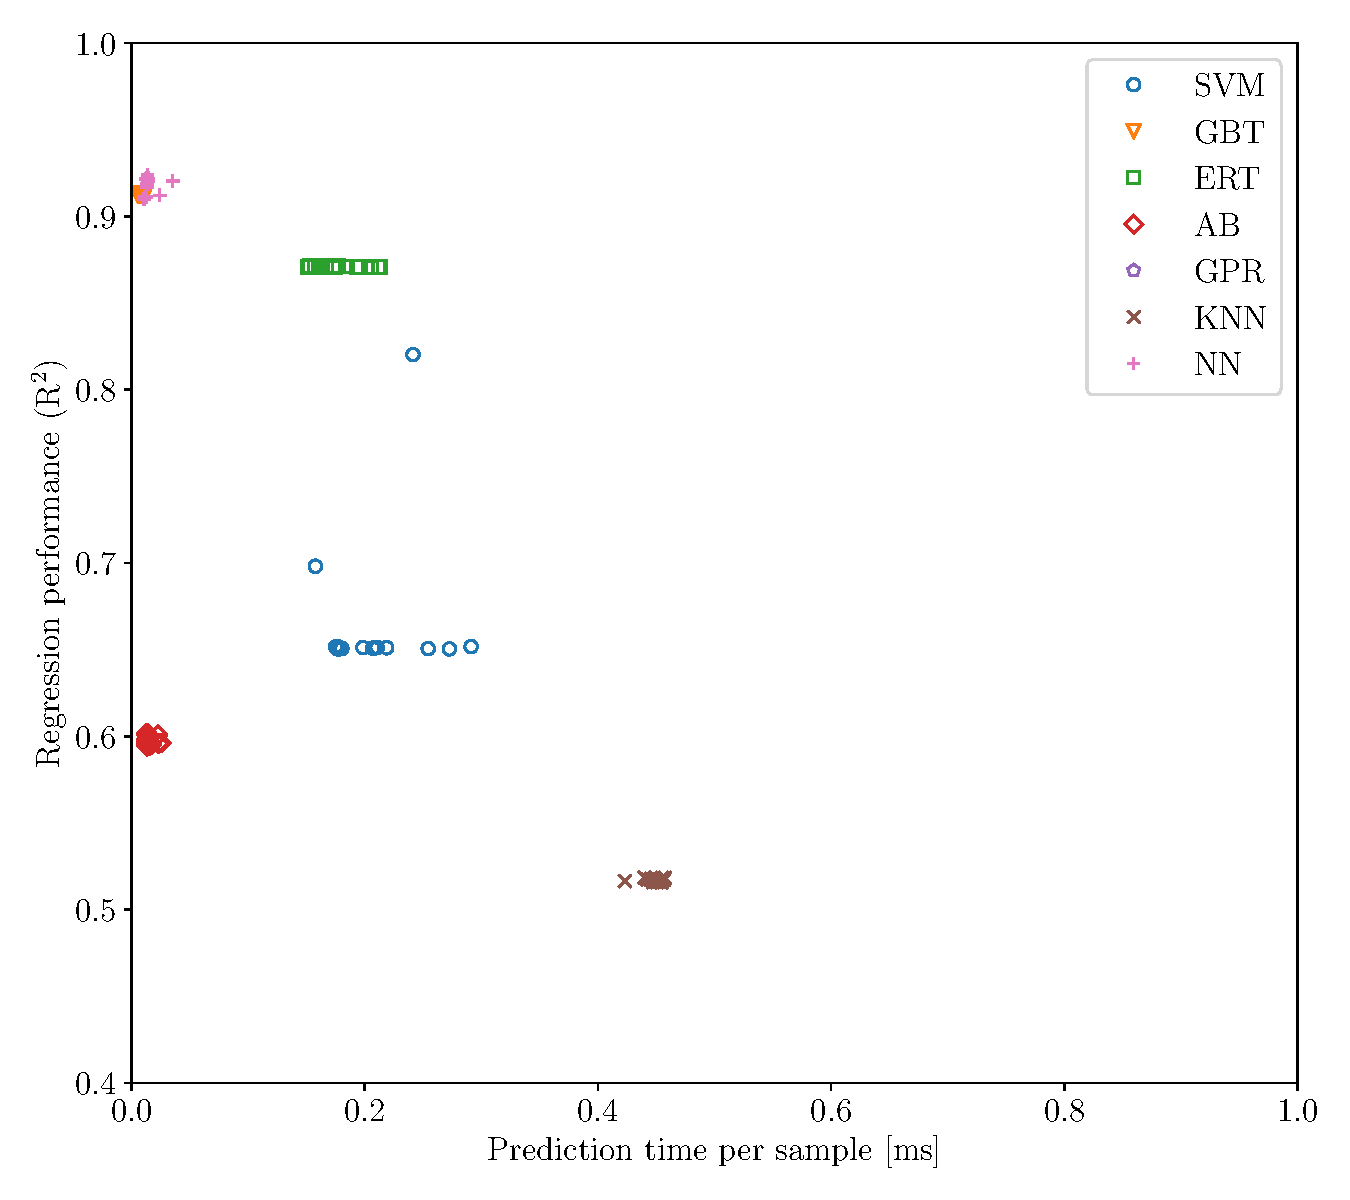
\includegraphics[width=\linewidth]{exp2_time_vs_reg}
	\caption{Results of experiment~2, plotted analogously
	to~\cref{fig:exp1-time-vs-reg}.}
	\label{fig:exp2-time-vs-reg}
\end{wrapfigure}

Following both hyperparameter tuning experiments, we conclude that while domain
restrictions employed in the first case have proven effective in improving the
regression performance of some methods, this result has fluctuated considerably
depending on the selected slices. Furthermore, in all instances the best
results were achieved by families of surrogates that were nearly unaffected by
this modification.


\subsubsection{Scaling Benchmark}

In the third experiment we examine surrogate scaling properties by correlating
metrics of interest with training set size. First, the results shown 
in~\cref{fig:scaling-r2} suggest that the most accurate families from the previous experiments
consistently maintain their relative advantage over others, even as we introduce
more training data. While such families achieve nearly comparable regression
performance on the largest dataset, in the opposite case methods based on
decision trees clearly outperform neural networks. This can be observed
particularly on training sets of sizes up to~\num{6000}.

\begin{figure}[h]
	\centering
	\begin{subfigure}[b]{0.333\textwidth}
		\centering
		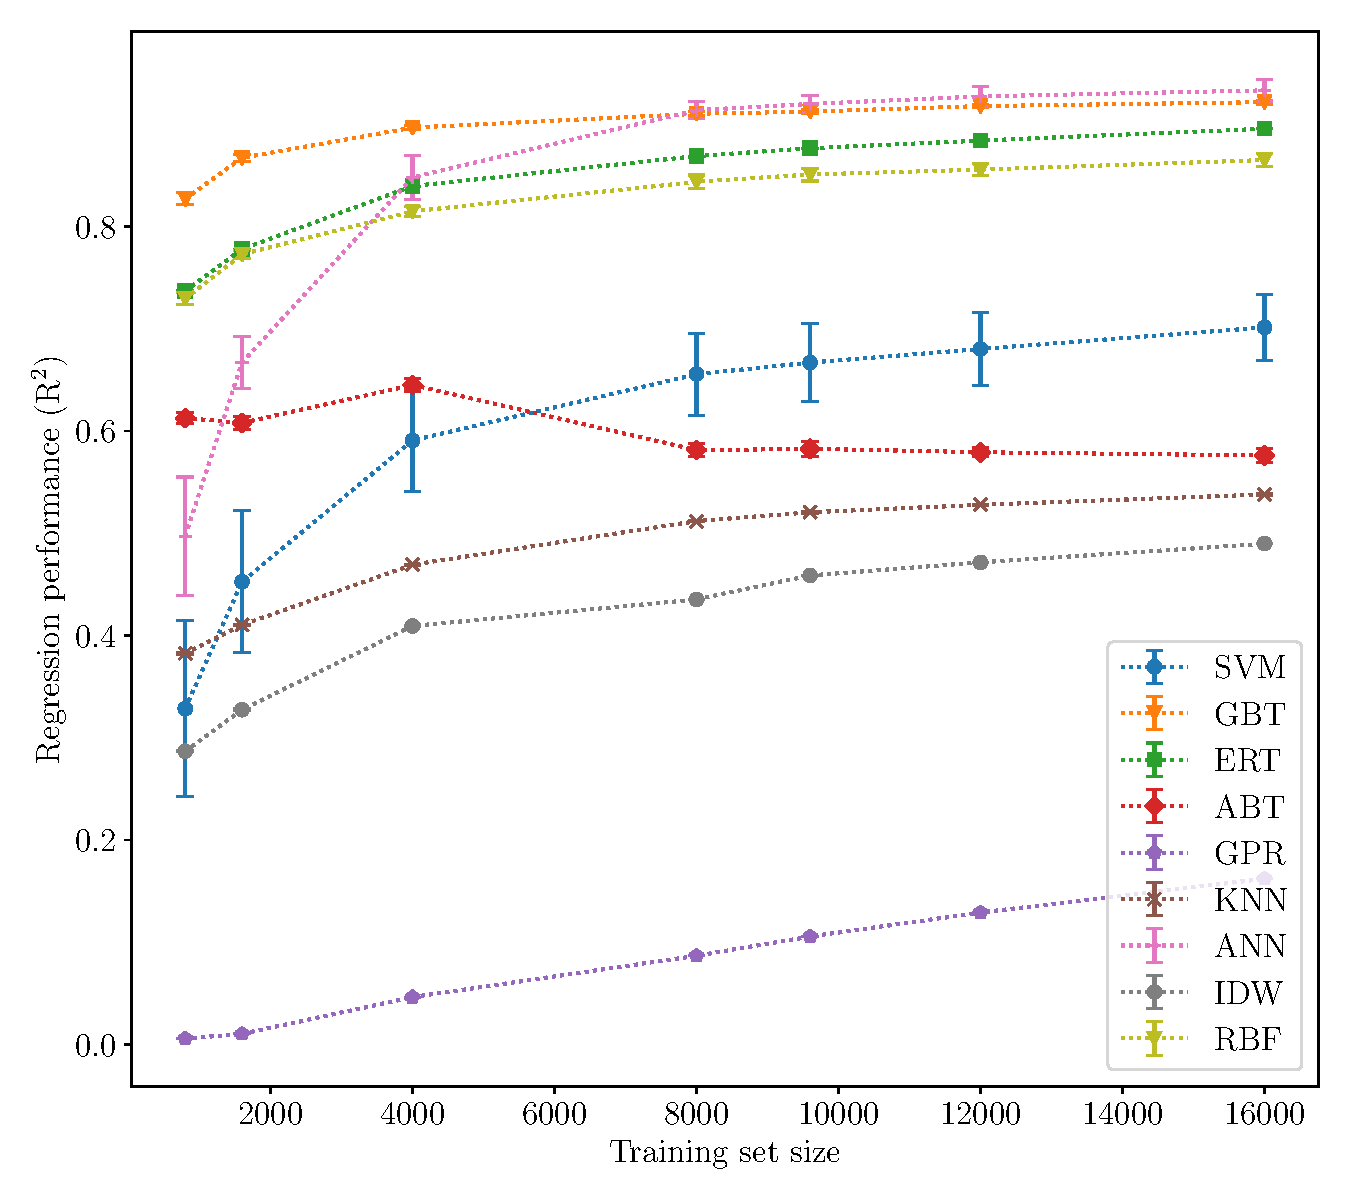
\includegraphics[width=\linewidth]{scaling_metric_r2}
		\caption{Regression performance (as $R^2$)}
		\label{fig:scaling-r2}
	\end{subfigure}\hfill%
	\begin{subfigure}[b]{0.333\textwidth}
		\centering
		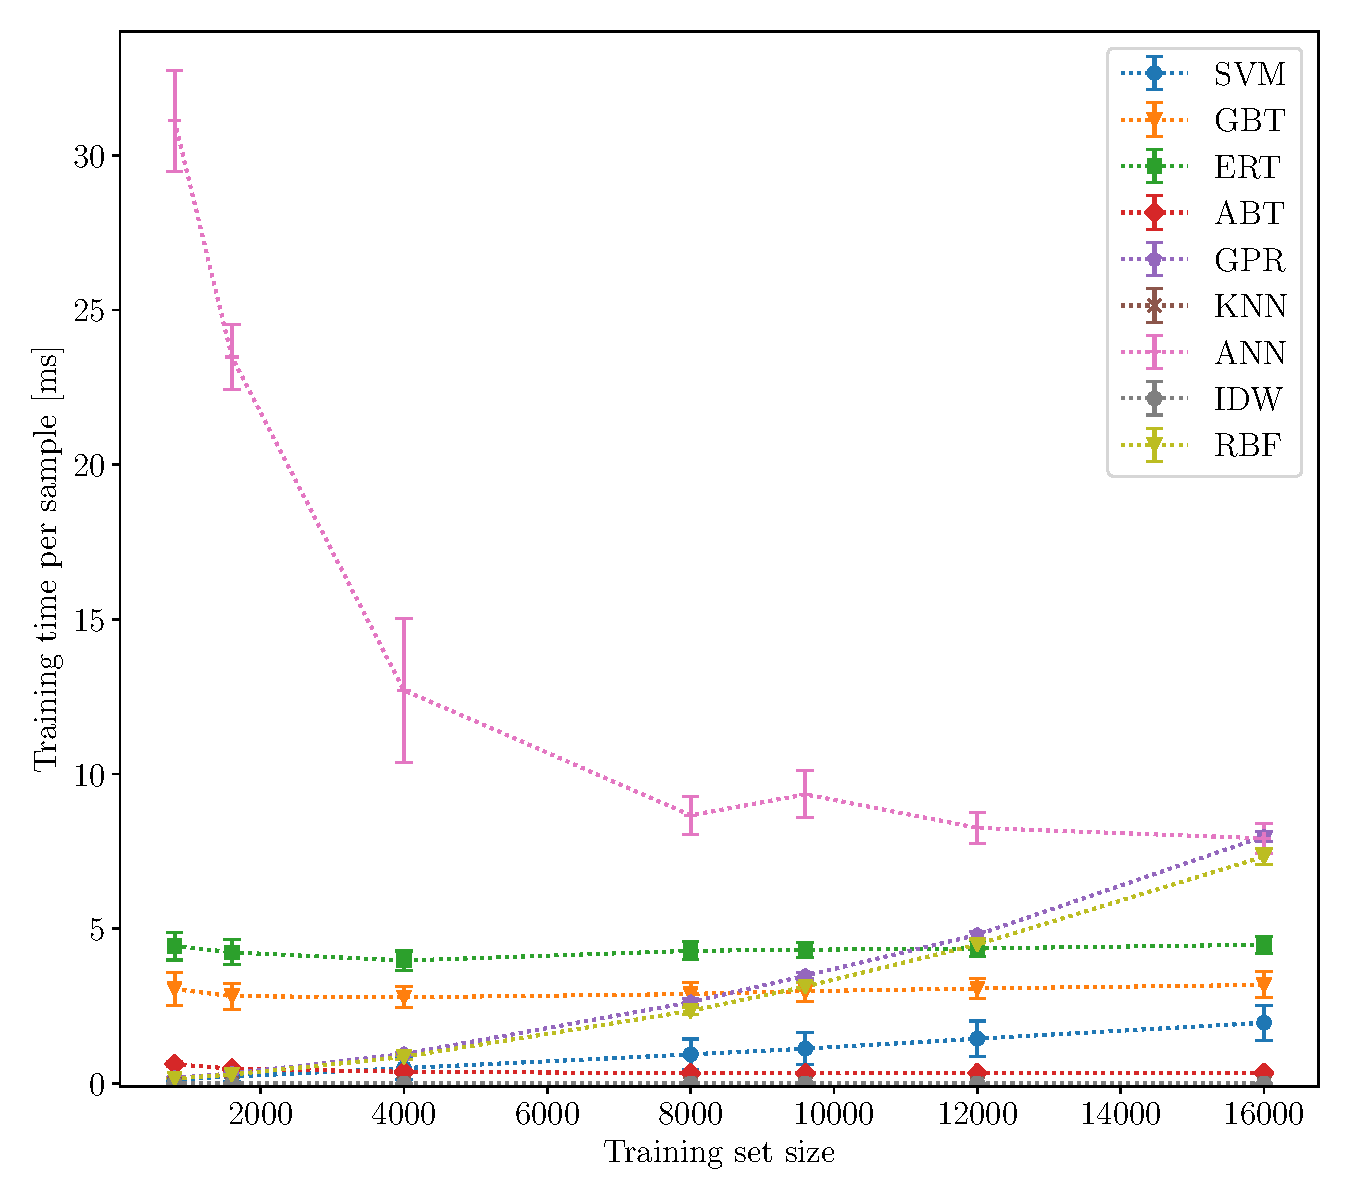
\includegraphics[width=\linewidth]{scaling_time_train}
		\caption{Complexity (as~$\overline{t}_{\text{trn.}}$)}
		\label{fig:scaling-trn}
	\end{subfigure}\hfill%
	\begin{subfigure}[b]{0.333\textwidth}
		\centering
		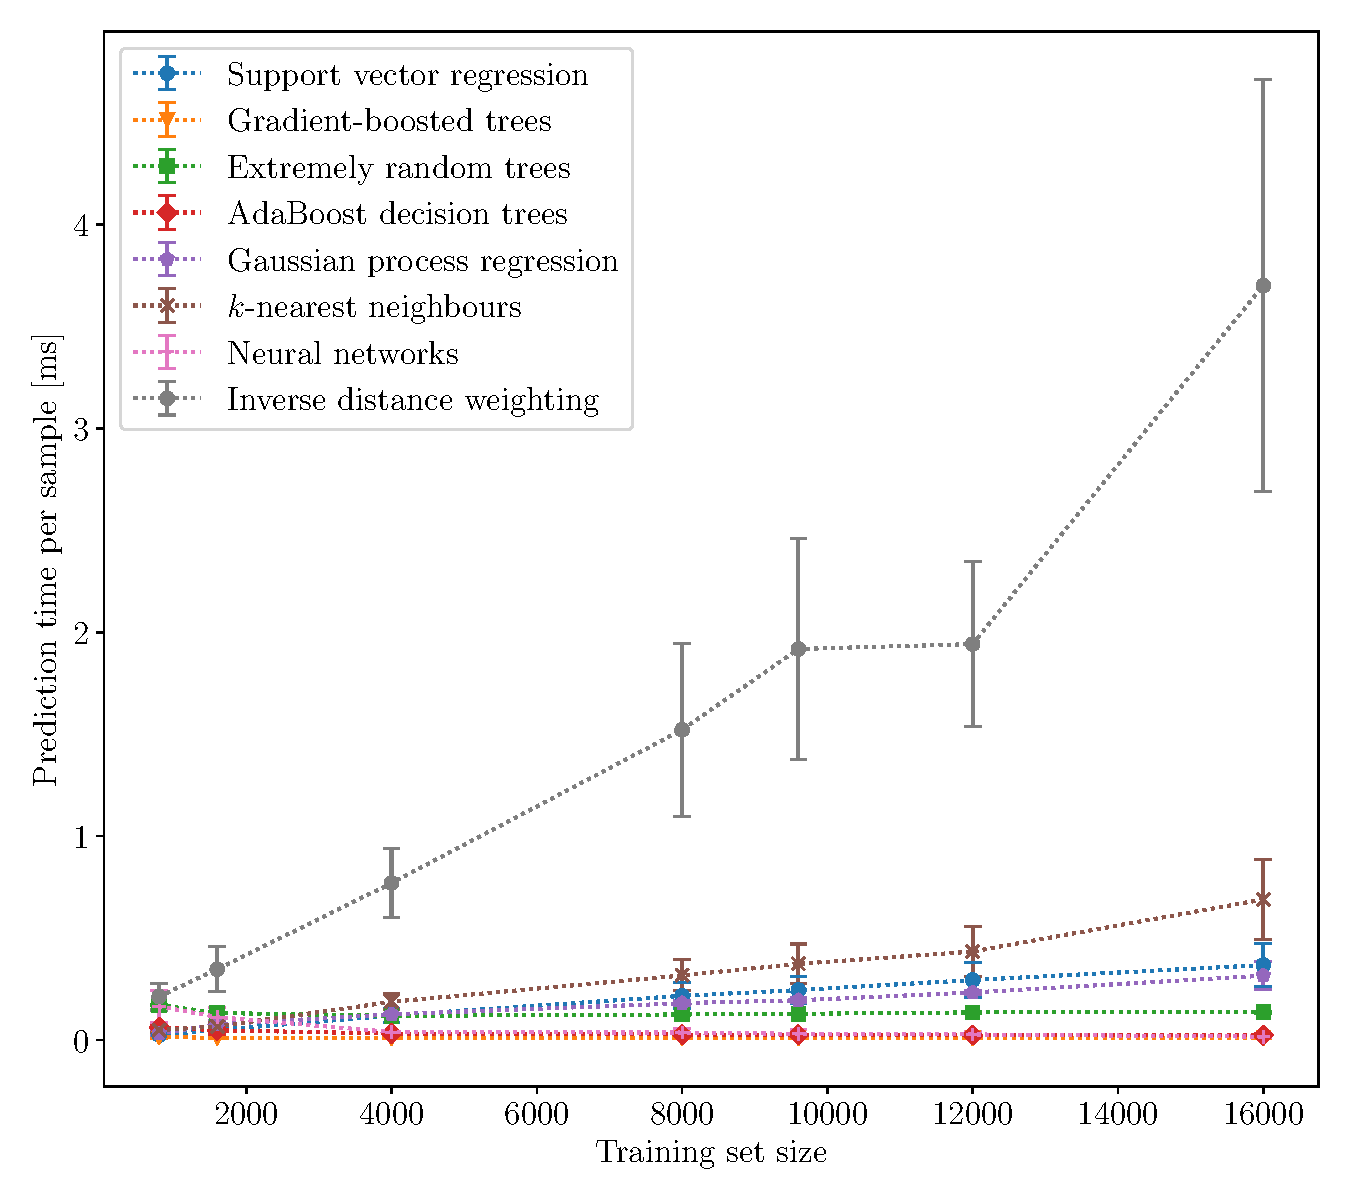
\includegraphics[width=\linewidth]{scaling_time_pred}
		\caption{Complexity (as~$\overline{t}_{\text{pred.}}$)}
		\label{fig:scaling-pred}
	\end{subfigure}
	\caption{Various metrics collected during experiment 3 (scaling
	benchmark) displayed as a function of training set size.}
	\label{fig:scaling}
\end{figure}

Next, we examine scaling behaviour in terms of the mean training time (displayed
in~\cref{fig:scaling-trn}). Consistent with our expectation, the shortest times
were achieved by instance-based learning methods (e.g. KNN, IDW) that
are trained trivially at the expense of increased lookup complexity later during prediction.
Furthermore, we observe that the majority of tree-based algorithms also exhibit
desirable properties unlike RBFs and gaussian process
regression, which appear to scale superlinearly. We note that ANNs,
which are the only family to utilise parallelisation during training, show an
inverse scaling characteristic. Our conjecture is that this effect may be caused
by a constant multi-threading overhead that possibly dominates the training process
on relatively small training sets.

Lastly, we study scaling with respect to the mean prediction time (shown
in~\cref{fig:scaling-pred}). Our initial observation is that all tested
surrogate families with the exception of previously mentioned instance-based
learning methods offer desirable characteristics overall. Analogous to previous
experiments, GBTs and ANNs again
appear to be tied, as they not only exhibit comparable times but also similar
scaling slopes.


\subsubsection{Model Comparison}

In the fourth and final experiment, we exploit previously collected information
to produce surrogates with desirable properties for practical use. We
aim to create models that yield: (i)~the best regression performance regardless
of other features, (ii)~acceptable performance with the shortest mean
prediction time, or (iii)~acceptable performance with the smallest training set.
To this end, we trained 8~surrogates that are presented in~\cref{fig:reg-performance}
(more details are given in~\cref{tbl:exp4-detailed-results} in the Appendix).

\begin{figure}[h]
	\centering
	\begin{subfigure}[b]{0.25\textwidth}
		\centering
		\includegraphics[width=\linewidth]{exp4_model1}
	\end{subfigure}\hfill%
	\begin{subfigure}[b]{0.25\textwidth}
		\centering
		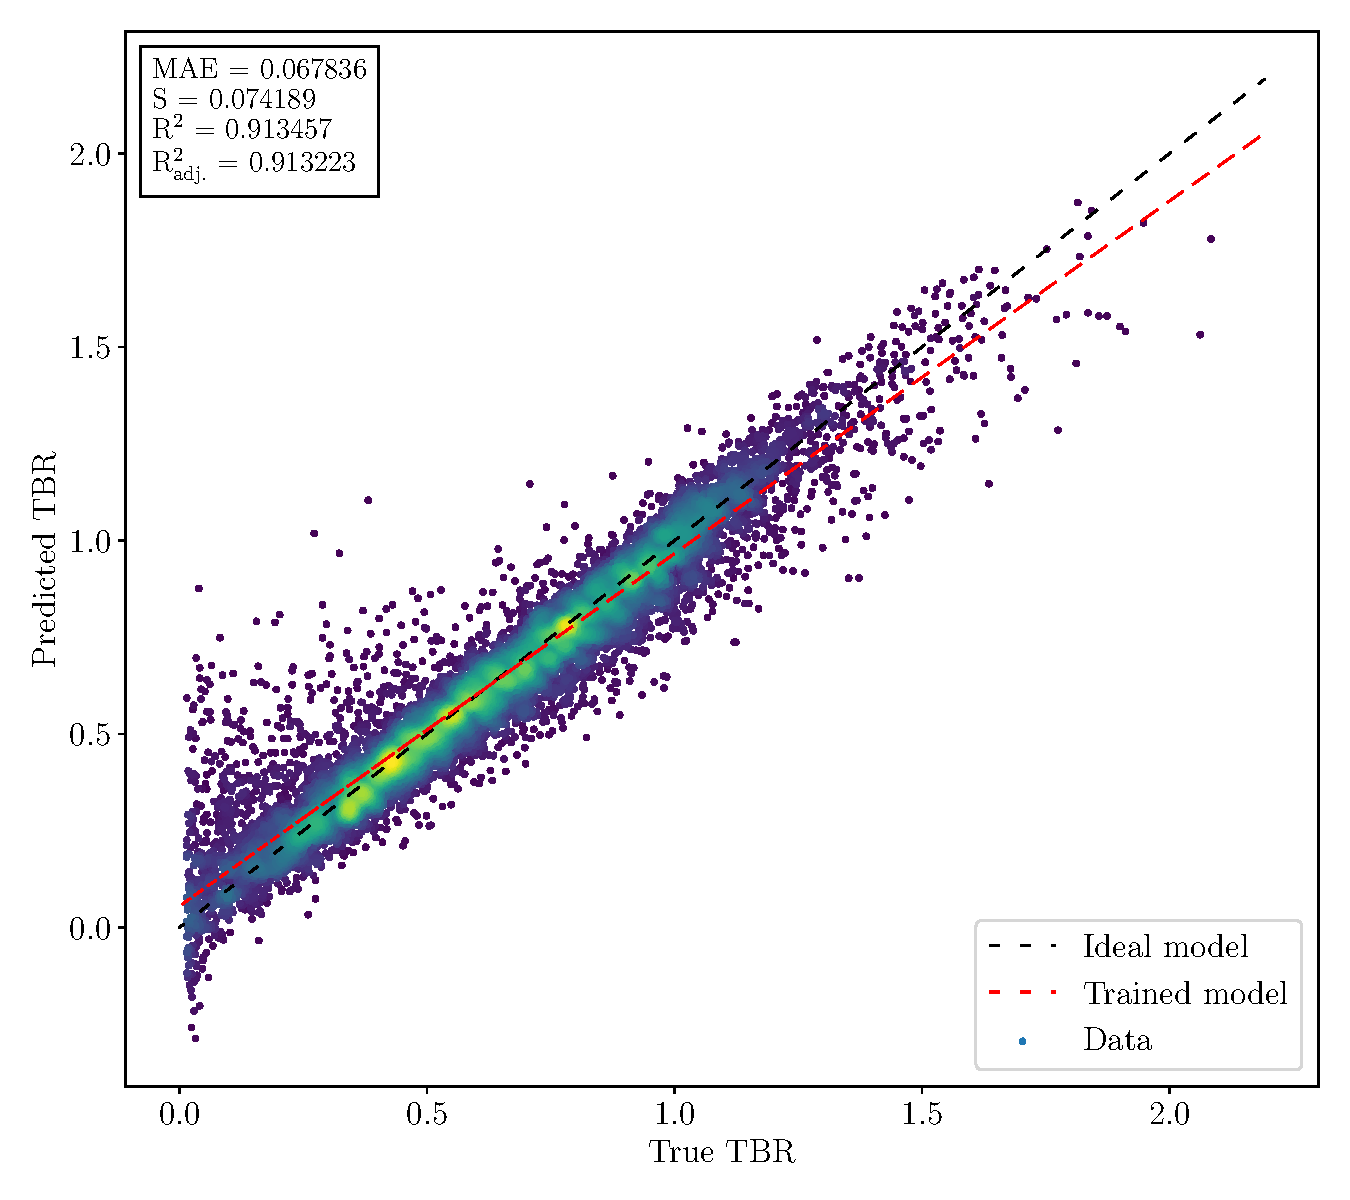
\includegraphics[width=\linewidth]{exp4_model2}
	\end{subfigure}\hfill%
	\begin{subfigure}[b]{0.25\textwidth}
		\centering
		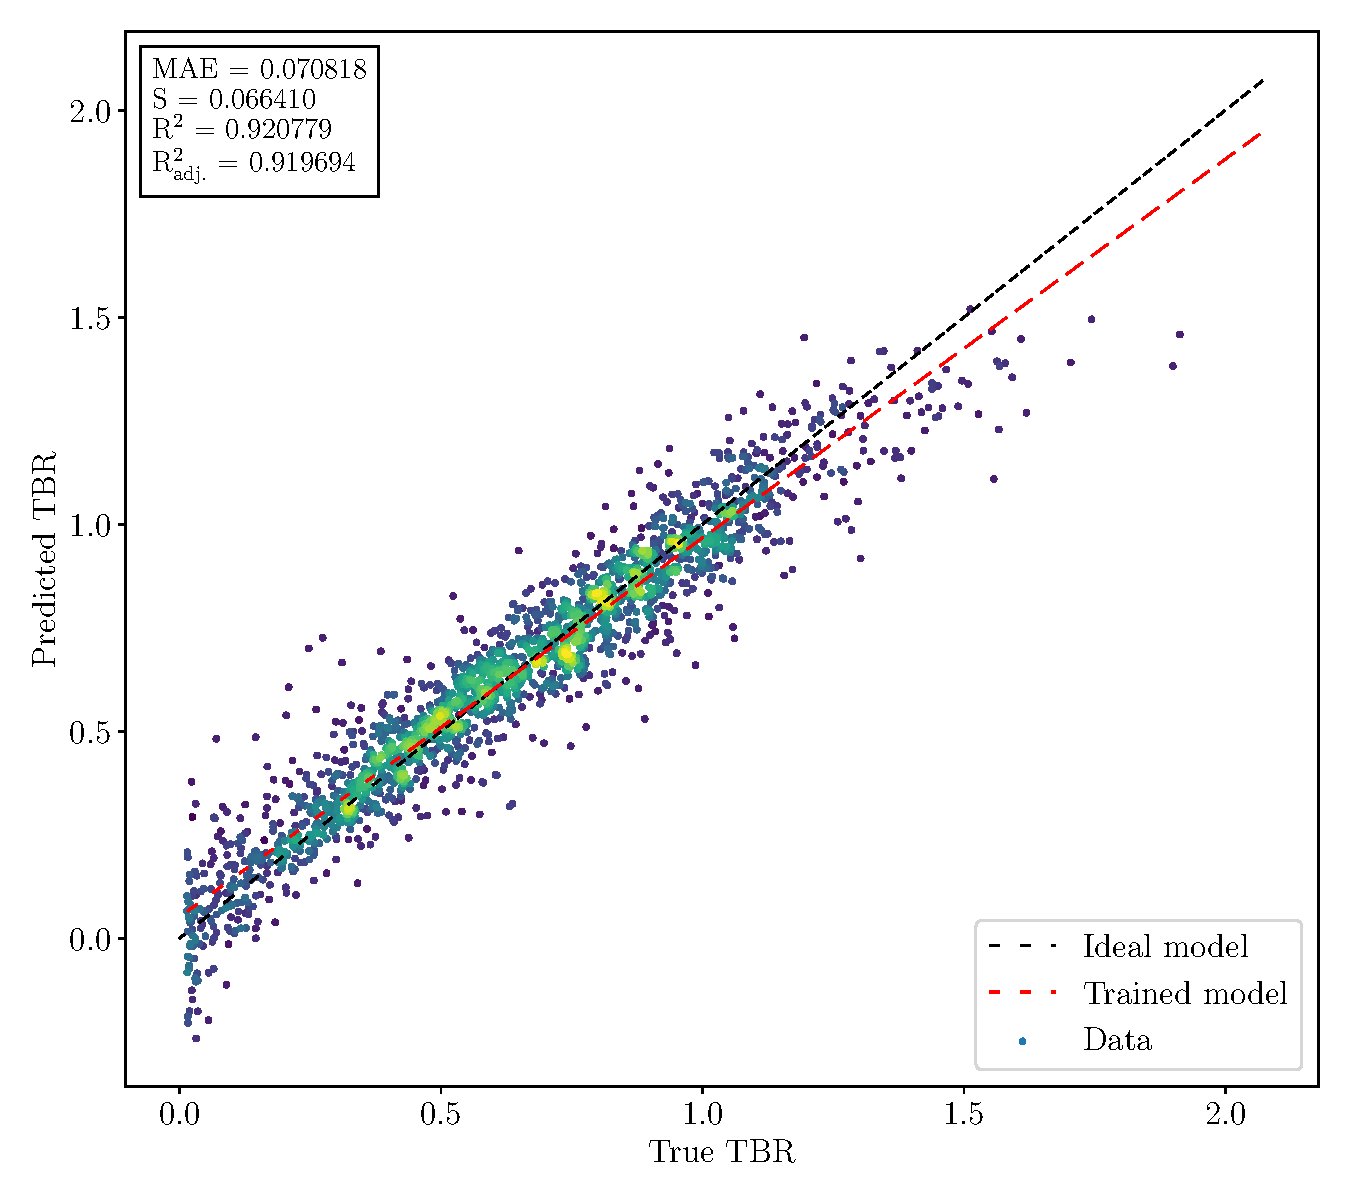
\includegraphics[width=\linewidth]{exp4_model3}
	\end{subfigure}\hfill%
	\begin{subfigure}[b]{0.25\textwidth}
		\centering
		\includegraphics[width=\linewidth]{exp4_model4}
	\end{subfigure}

	\begin{subfigure}[b]{0.25\textwidth}
		\centering
		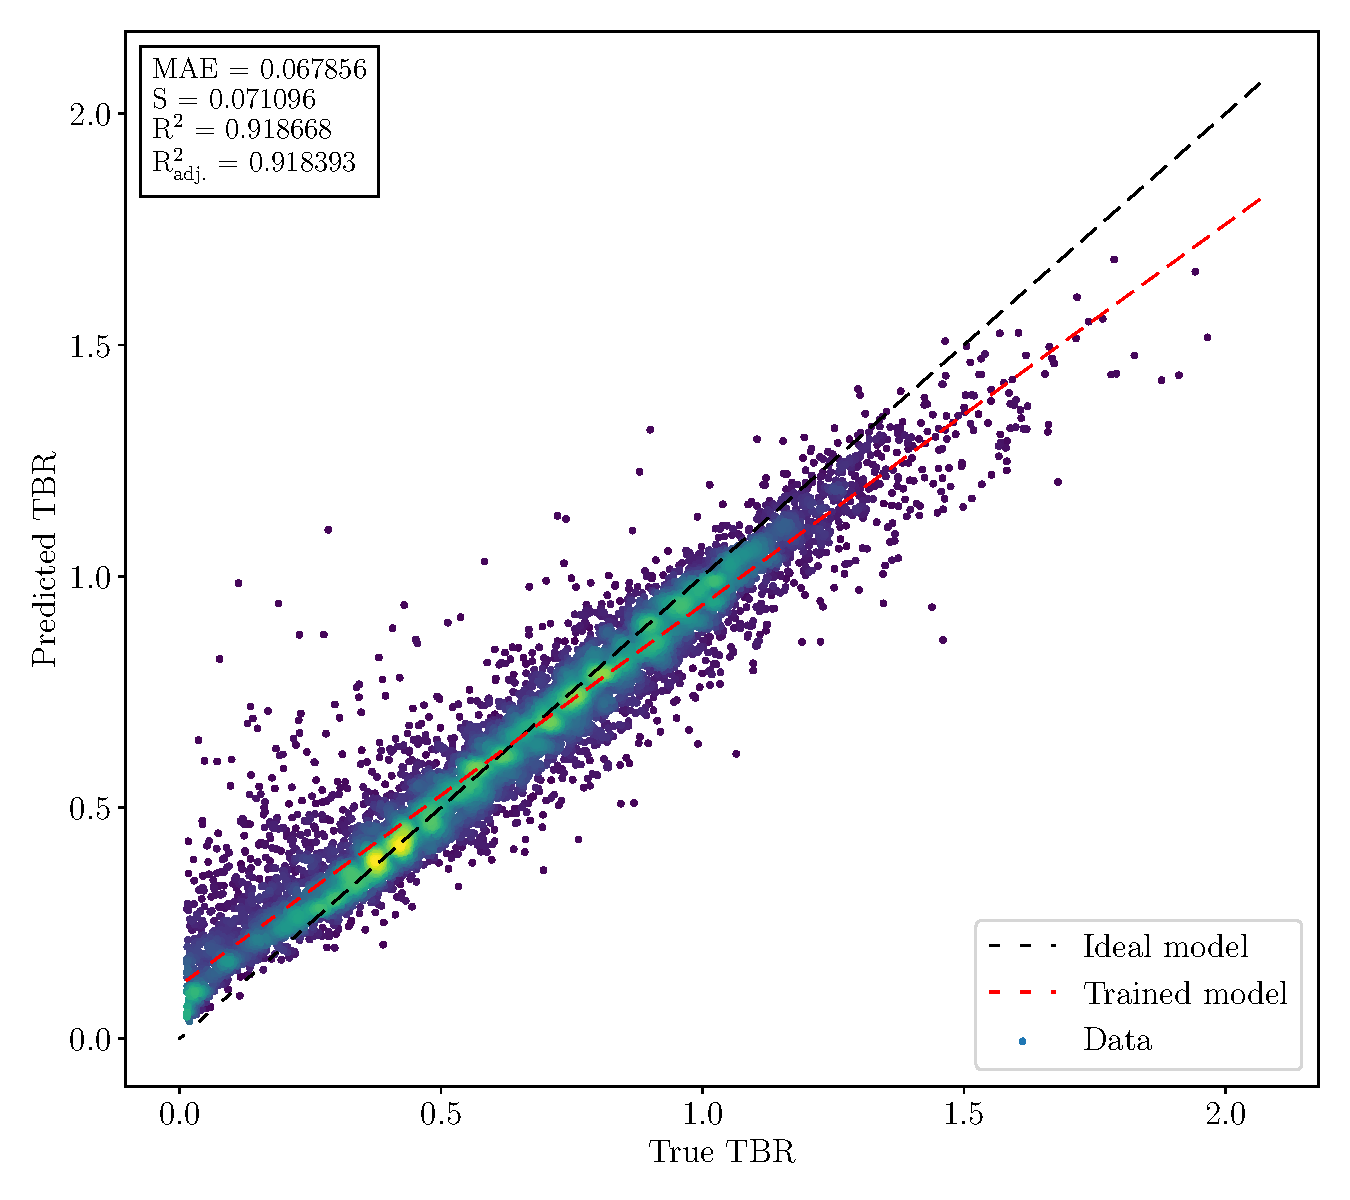
\includegraphics[width=\linewidth]{exp4_model5}
	\end{subfigure}\hfill%
	\begin{subfigure}[b]{0.25\textwidth}
		\centering
		\includegraphics[width=\linewidth]{exp4_model6}
	\end{subfigure}\hfill%
	\begin{subfigure}[b]{0.25\textwidth}
		\centering
		\includegraphics[width=\linewidth]{exp4_model7}
	\end{subfigure}\hfill%
	\begin{subfigure}[b]{0.25\textwidth}
		\centering
		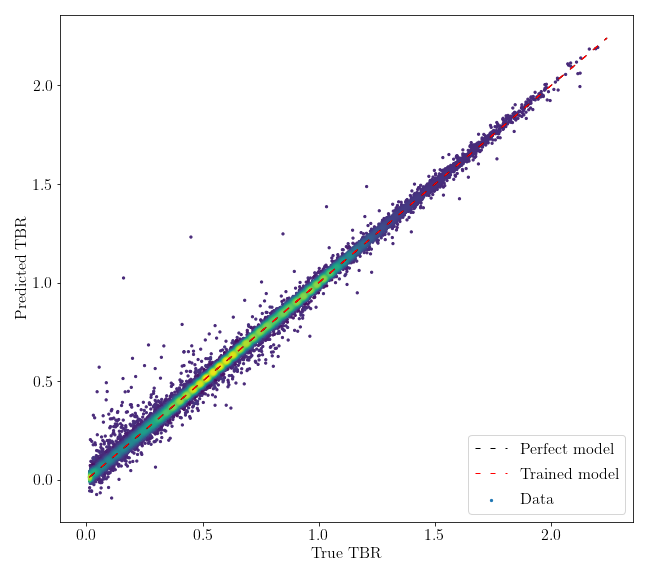
\includegraphics[width=\linewidth]{run1_5ke_1h3f128_4974_performance}
		% TODO: only a placeholder, regenerate when data becomes available
	\end{subfigure}
	\caption{Regression performance of models 1-4 (row 1, from the left) and 5-8
		(row 2) trained in experiment~4 (model comparison), viewed
		as true vs. predicted TBR on a test set of a selected cross-validation
		fold. Points are coloured by density.}
	\label{fig:reg-performance}
\end{figure}

Having selected ANNs, GBTs, ERTs, RBFs and SVMs based on the results of the
experiments~2-3, we utilised the best-performing hyperparameter
assignments and training sets of varying sizes. In attempts to satisfy
goals~(i) and~(ii) within cross-validation setting, our best surrogate
achieved~$R^2=\num{0.998}$ and mean prediction
time~$\overline{t}_{\text{pred.}}=\SI{0.898}{\micro\second}$. These correspond
to the standard error of regression~$S=\num{0.013}$ and a relative speedup~$\omega=\num{8659251} \times$
with respect to the MC TBR evaluation baseline measured during run~1
(see~\cref{tbl:sampling-runs} for details). While this particular surrogate
was trained on the entire available set of~\num{500000} datapoints, in attempts to satisfy
goal~(iii) we also trained a more simplified model that achieved~$R^2=\num{0.913}$,
$\overline{t}_{\text{pred.}}=\SI{6}{\micro\second}$, $S=\num{0.072}$ and $\omega=\num{1269777} \times$
with only a set of size~\num{10000}.

Overall we found that due to their excellent performance, boosted tree-based
approaches seem to be advantageous for fast surrogate modelling on relatively small training
sets (up to the order of~$10^4$). Conversely, while neural networks perform
poorly in such a setting, both their regression performance and prediction times
have proven superior on larger training sets (at least of the order of~$10^5$).


\begin{wrapfigure}[13]{r}{0.4\textwidth}
	\centering
	\vspace{-12ex}
	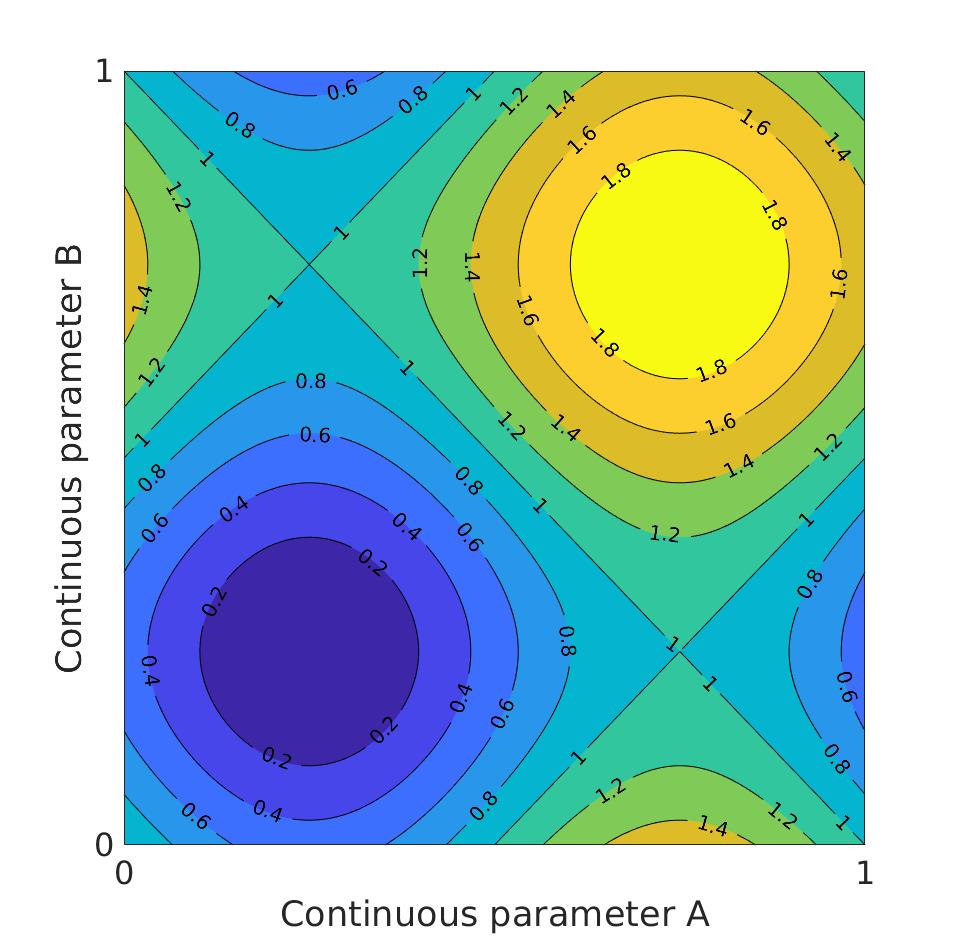
\includegraphics[width=0.4\textwidth]{fig5_sintoy.jpg}
	\caption{Sinusoidal toy TBR theory over two continuous parameters, wavenumber 1}
	\label{fig:sintoy}
\end{wrapfigure}

\subsection{Results of Adaptive Sampling}
\label{sec:adaptiveres}

In order to test our QASS prototype, several functional toy theories for TBR were developed as alternatives to the expensive MC model. By far the most robust of these was the following sinusoidal theory with adjustable wavenumber parameter $n$:

\begin{equation}
	\text{TBR} = \text{Mean}_{i \in C} \left[ \frac{1 + \sin(2\pi n (x_i - 1/2)) }{2} \right]
\end{equation}

plotted in~\cref{fig:sintoy} for $n=1$ and two continuous parameters $C$. ANNs
trained on this model demonstrated similar performance to those on the expensive
MC model. QASS performance was verified by training a $\text{1h3f}(256)$ ANN on
the sinusoidal theory for varied quantities of initial, incremental, and MCMC
candidate samples. Although the scope of this project did not include thorough
searches of this hyperparameter domain, sufficient runs were made to identify
some likely trends.

An increase in MCMC candidate samples was seen to have a positive but very weak
effect on final surrogate precision, suggesting that the runtime of MCMC on each
iteration can be limited for increased efficiency. -- Awaiting test results on
initial sample quantity --. The most complex dynamics arose with the adjustment
of sample increment, shown in~\cref{fig:qassincr}. For each tested initial sample quantity N, the optimal number of step samples was seen to be well-approximated by $\sqrt{N}$; the plotted error trends suggest that incremental samples larger than this optimum give slower model improvement on both the training and evaluation sets, and a larger minimum error on the evaluation set. This performance distinction is predicted to be even more significant when trained on the expensive MC model, where the number of sample evaluations will serve as the primary bottleneck for computation time.
\begin{figure}[h!]
    \centering
    \begin{subfigure}[t]{0.5\textwidth}
        \centering
        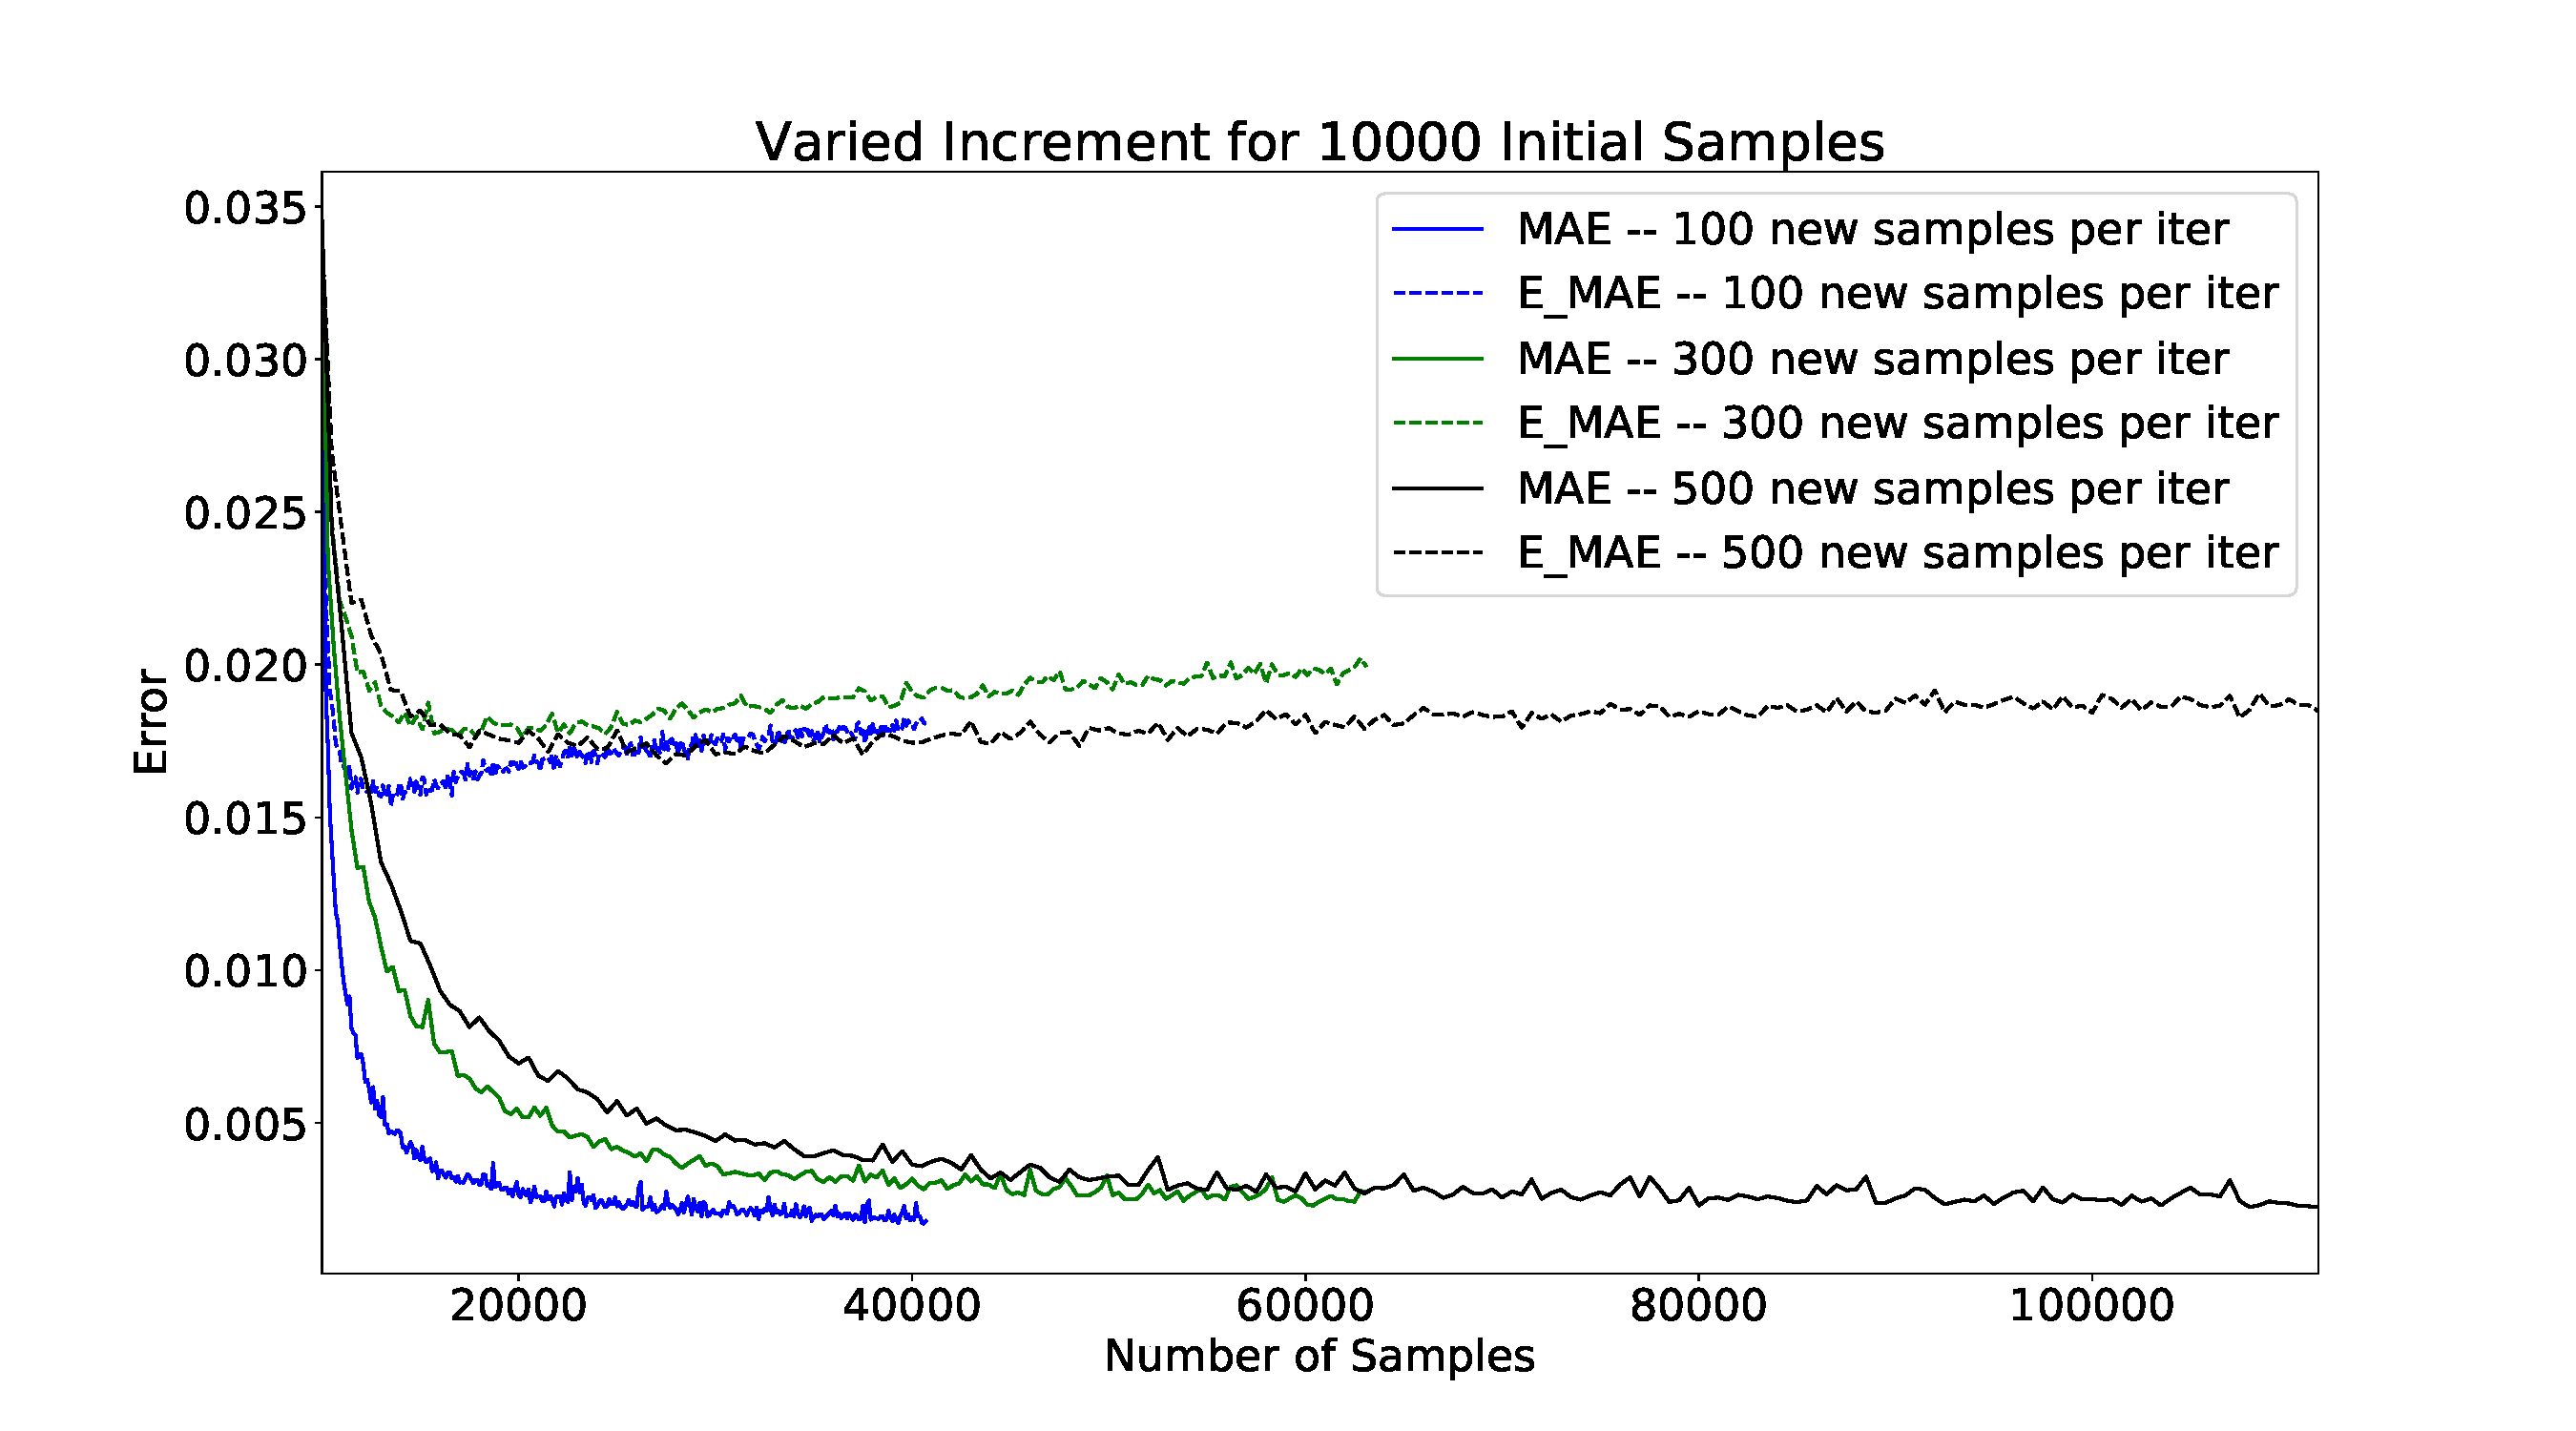
\includegraphics[width=1.1\linewidth]{fig6a_qassincrsamp.pdf}
    \end{subfigure}%
    \hfill
    \begin{subfigure}[t]{0.5\textwidth}
        \centering
        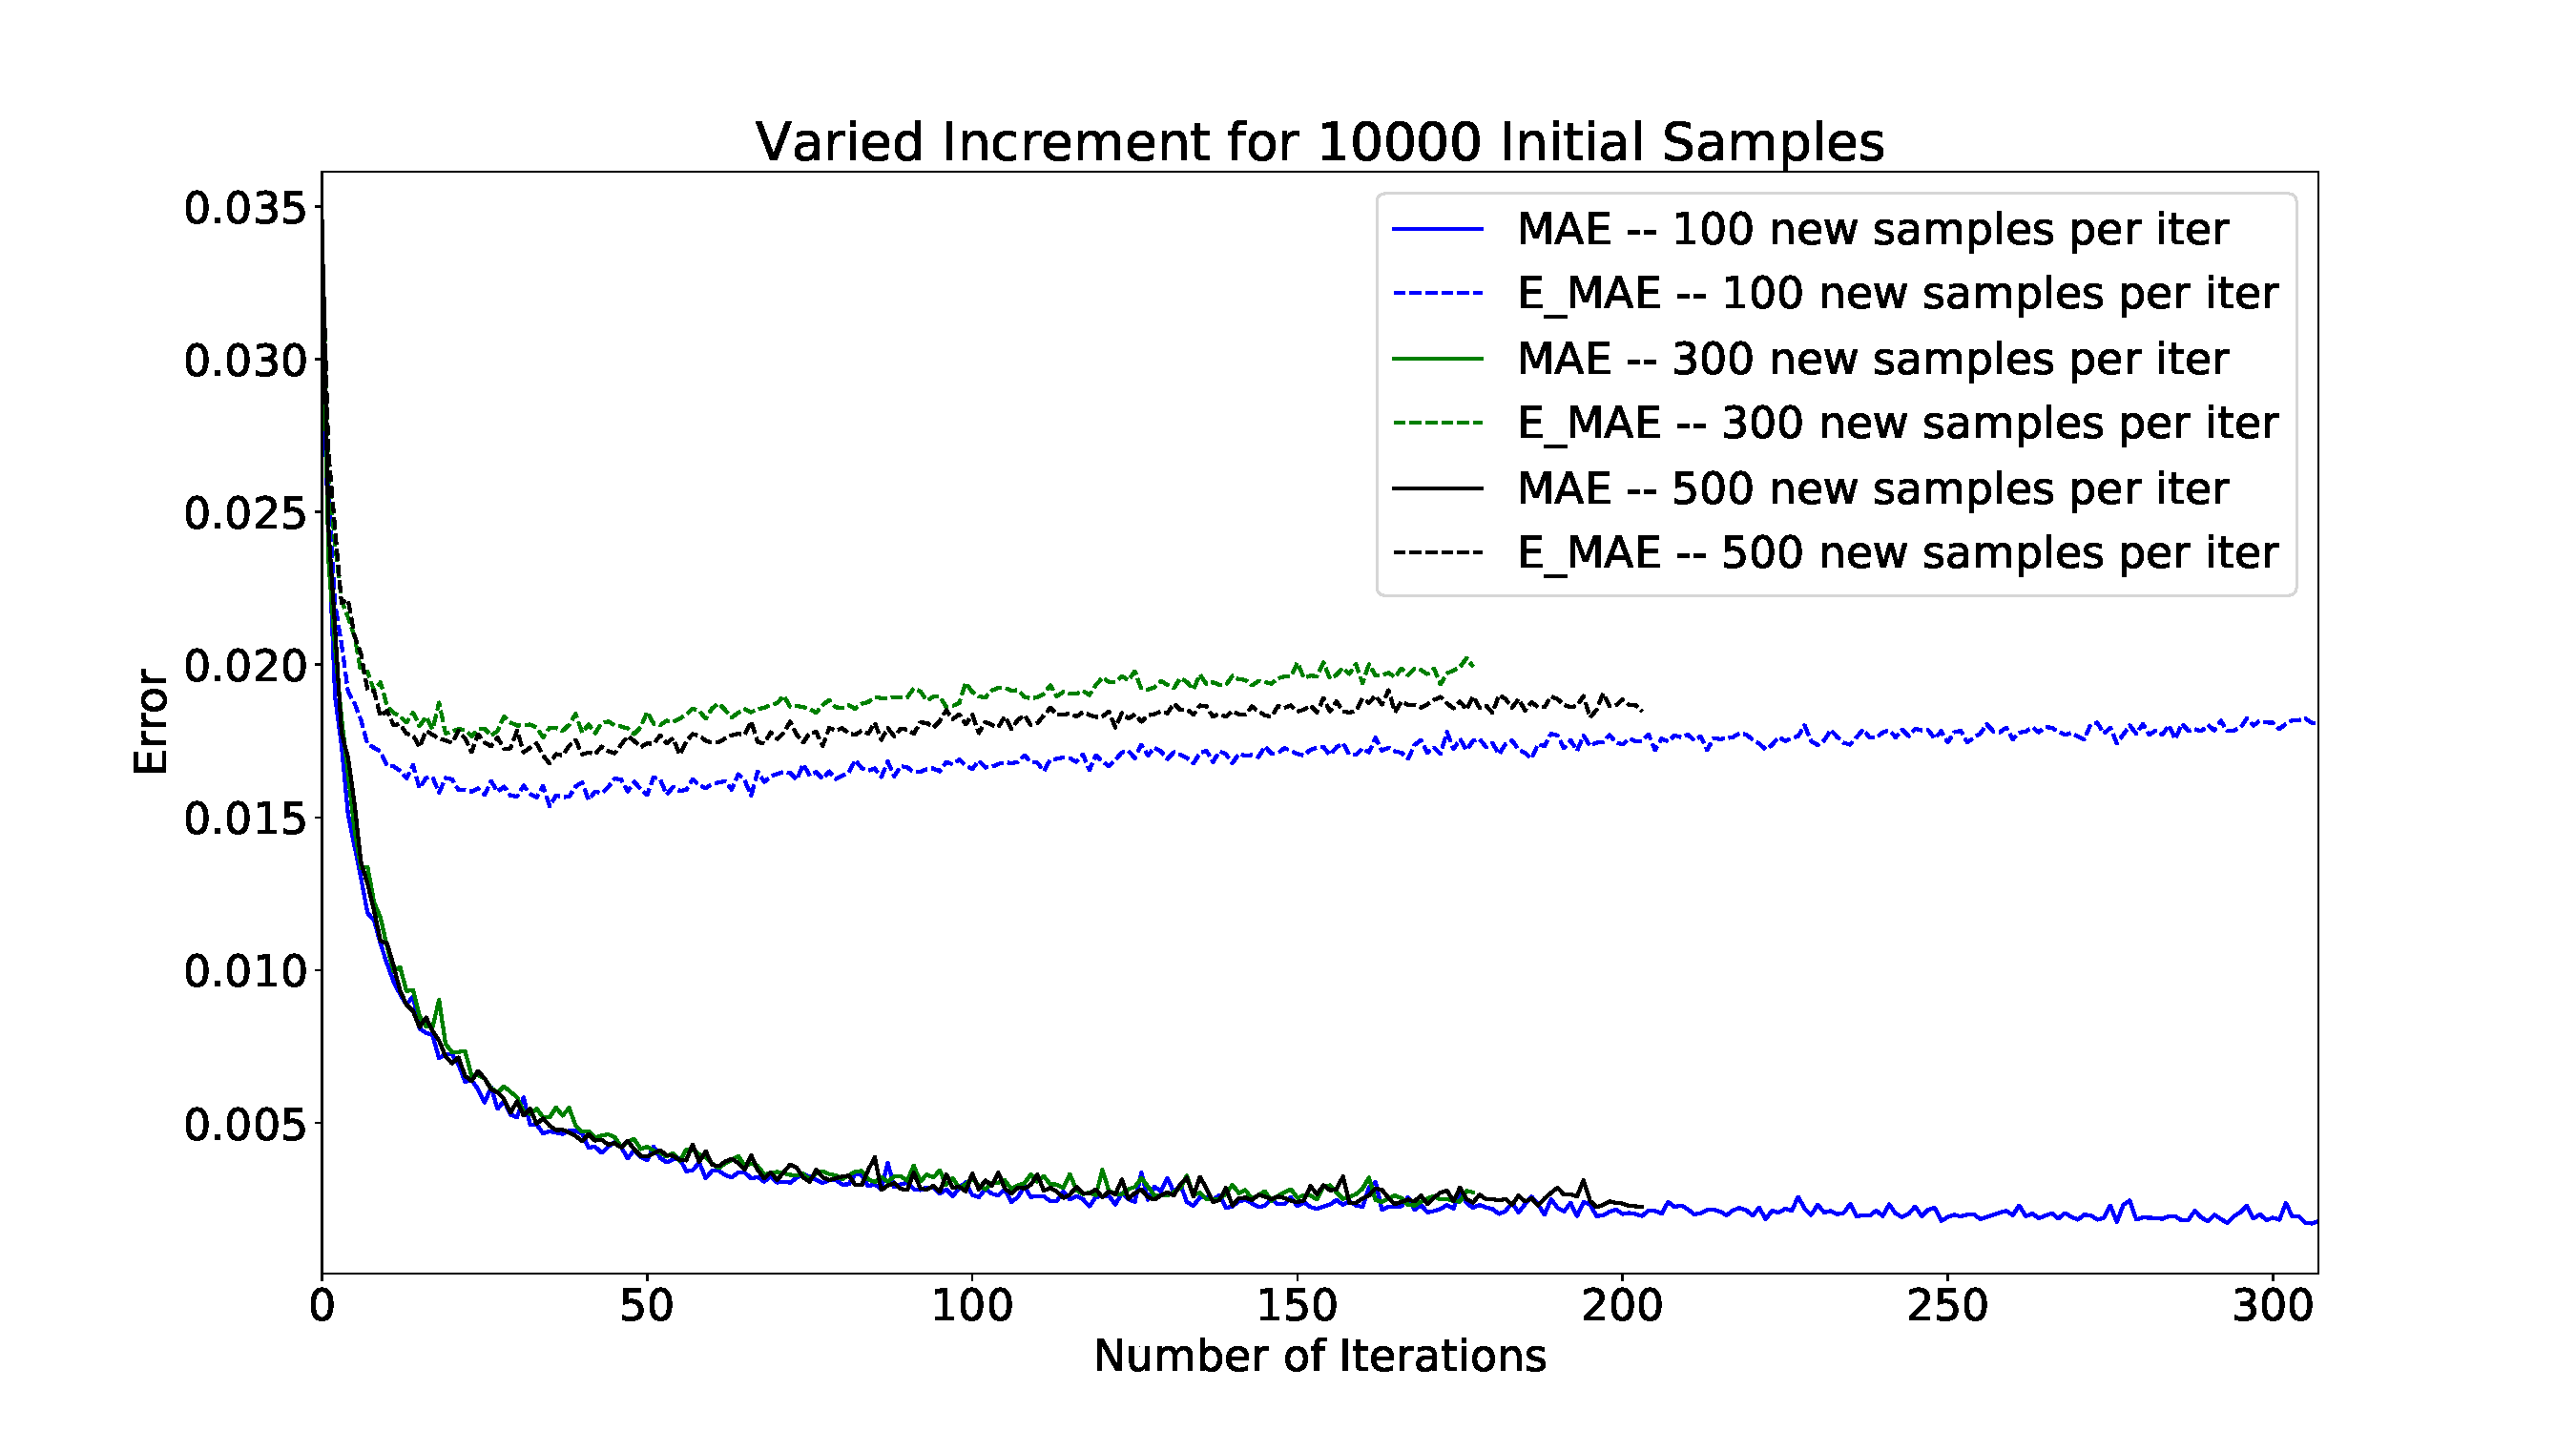
\includegraphics[width=1.1\linewidth]{fig6b_qassincrtime.pdf}
    \end{subfigure}
    \caption{QASS absolute training error over total sample quantity (left) and number of iterations (right). MAE represents surrogate error on the adaptively-sampled training/test set, and E\_MAE on the independent evaluation sets.}
    \label{fig:qassincr}
\end{figure}

The plateau effect in surrogate error on the evaluation set, seen
in~\cref{fig:qassincr}, was universal to all configurations and thought to
warrant further investigation. At first this was suspected to be a residual
effect of retraining the same ANN instance without adjustment to data
normalisation; a "Goldilocks scheme" for checking normalisation drift was
implemented and tested, but did not affect QASS performance. Schemes in which
the ANN is periodically retrained were also discarded, as the retention of
network weights from one iteration to the next was demonstrated to greatly
benefit QASS efficiency. Further insight came from direct comparison between
QASS and a baseline scheme with uniformly random incremental samples, shown
in~\cref{fig:qasssampling}.

\begin{figure}[h]
  \centering
    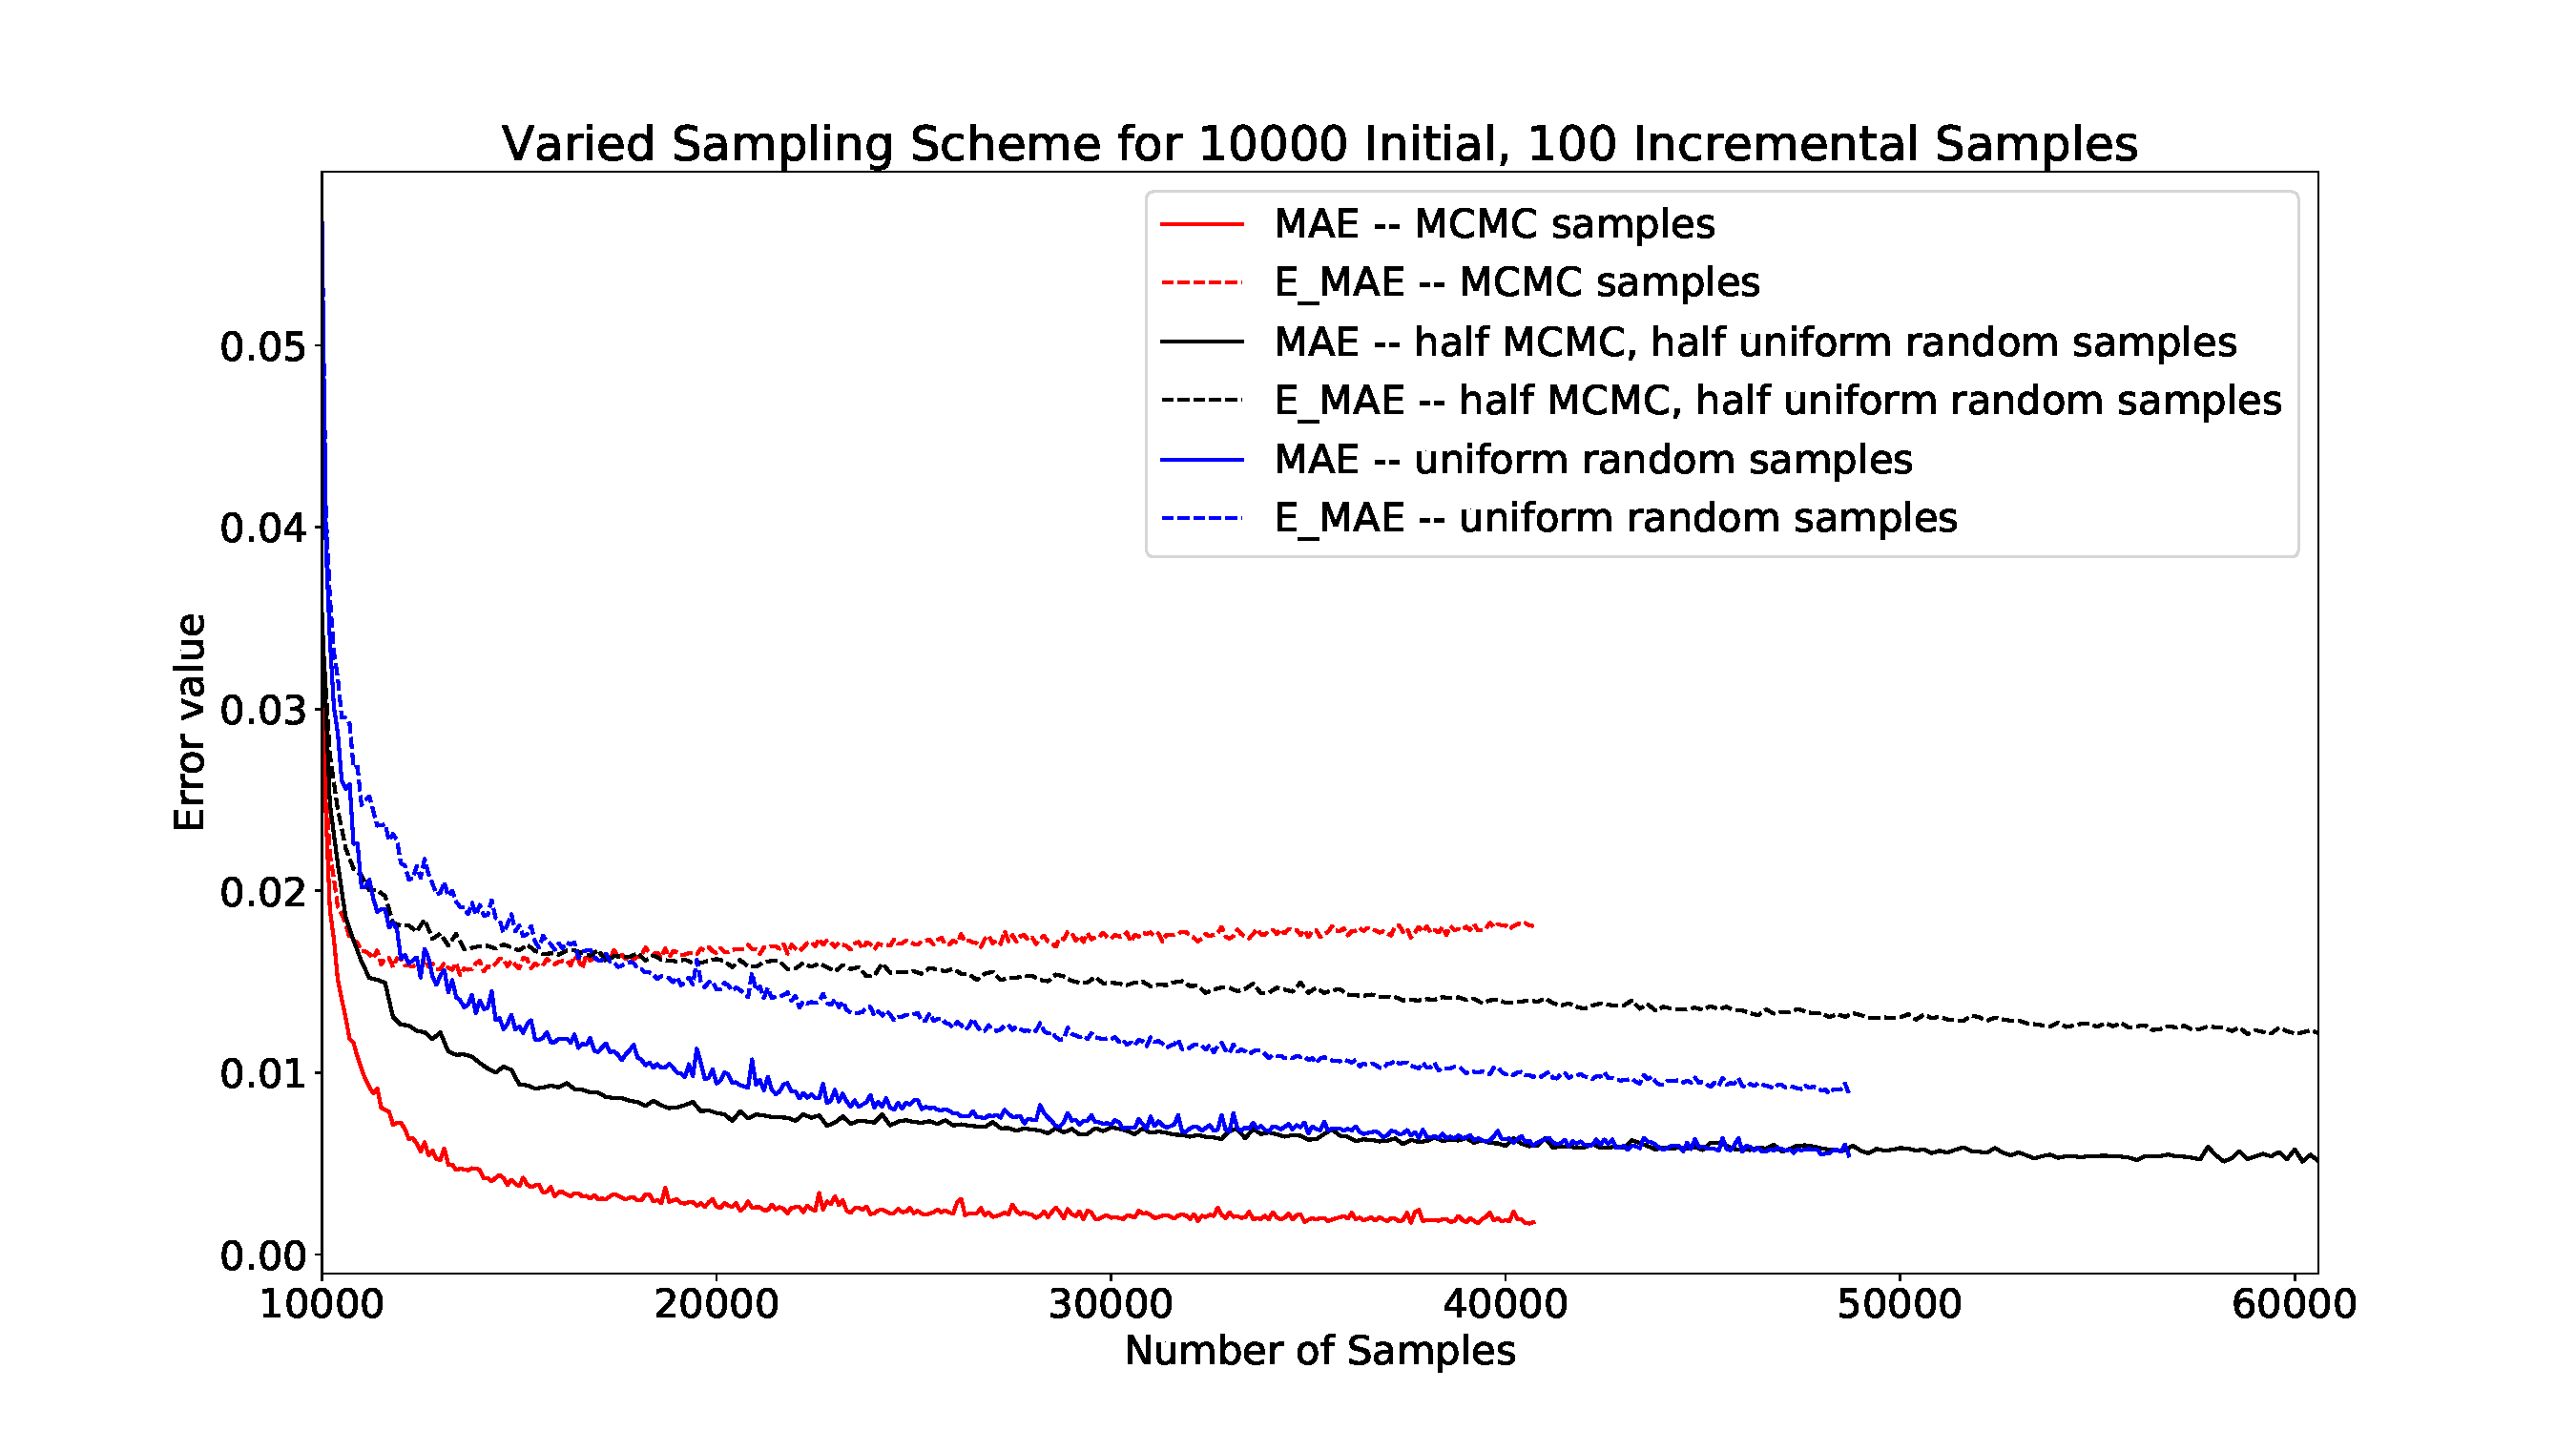
\includegraphics[width=0.78\linewidth]{fig7_qasssampling.pdf}
    \caption{Absolute training error for QASS, baseline scheme, and mixed scheme}
  \label{fig:qasssampling}
\end{figure}

Such tests revealed that while QASS has unmatched performance on its own
adaptively-sampled training set, it is outperformed by the baseline scheme on
uniformly random evaluation sets. We suspected that while QASS excels in
learning the most strongly peaked regions of the TBR theory, this comes at the
expense of precision in broader, smoother regions where uniformly random
sampling suffices. Therefore a mixed scheme was implemented, with half MCMC
samples and half uniformly random samples incremented on each iteration, which
is also shown in~\cref{fig:qasssampling}.

%---------------------------------------------------------------------

\section{Conclusion}
\label{sec:conclusion}
Over the course of this internship project, we employed a broad spectrum of data
analysis and machine learning techniques to develop fast and high-quality
surrogates for a~MC TBR model in use at~UKAEA. We generated over~\num{900000}
samples for training and test purposes, evaluated on this expensive MC~model. We
investigated possibilities for simplification of the parameter space, and
concluded that no straightforward reduction was possible. After reviewing
9~surrogate model families, examining their behaviour on constrained and
unrestricted feature space, and studying their scaling properties, we retrained
some of the best-performing instances to produce properties desirable for
practical use. The best approximator, trained on~\num{500000} datapoints,
featured~$R^2=\num{0.998}$ with mean prediction time
of~$\SI{0.898}{\micro\second}$, representing a relative
speedup~$\num{8659251} \times$ with respect to the MC model. Alternatively, we
also demonstrated the possibility of achieving comparable results using only a
training set of size~\num{10000}.

After a thorough review of the literature, we developed a novel adaptive
sampling algorithm, QASS, capable of interfacing with any of the individual
studied models. Preliminary testing on a toy theory, qualitatively comparable to
the MC TBR model, demonstrated the effectiveness of QASS and behavioural trends
consistent with the design of the algorithm. \textit{[Insert numerical results
for QASS.]} Further optimisation over the hyperparameter space has strong
potential to increase this performance, allowing for future deployment of QASS
on the MC TBR model in coalition with any of the most effective identified
surrogate models.


\section*{Acknowledgements}

The authors would like to thank Vignesh Gopakumar, Prof.~Nikolaos
Konstantinidis, Nikolaos Nikolaou, Prof.~Emily Nurse, Jonathan Shimwell and Ingo
Waldmann for their supervision and valuable suggestions related to this work.


%---------------------------------------------------------------------

\nocite{*}
\begin{multicols}{2}[\section*{References}]
\printbibliography[heading=none]
\end{multicols}
%---------------------------------------------------------------------

\begin{appendices}
	\section{Detailed Results of Supervised Models}
	\label{app:detailed-results}
	\begin{table}[!hbt]
	\centering
	\sisetup{round-mode=places,round-precision=3}
	{\scriptsize
		\begin{tabular}{lrrrrrrr}
		\toprule
		{} & {} & \multicolumn{4}{c}{Regression performance} &
		\multicolumn{2}{c}{Complexity}\\
		\cmidrule(lr){3-6}
		\cmidrule(lr){7-8}
		Family & \# & MAE [TBR] & $S$ [TBR] & $R^2$ [rel.] & $R^2_{\text{adj.}}$ [rel.]
						& $\overline{t}_{\text{trn.}}$ [\si{\milli\second}] &
						$\overline{t}_{\text{pred.}}$ [\si{\milli\second}]\\
		\midrule
		
		SVM
						& \num{1040}
						& $\num{0.077909} \pm \num{0.012203}$
						& $\num{0.096007} \pm \num{0.013410}$
						& $\num{0.864927} \pm \num{0.030560}$
						& $\num{0.862165} \pm \num{0.031185}$
						& $\num{0.247436} \pm \num{0.014104}$
						& $\num{0.035208} \pm \num{0.006046}$
\\

		GBT
						& \num{1000}
						& $\num{0.061841} \pm \num{0.009911}$
						& $\num{0.061776} \pm \num{0.007628}$
						& $\num{0.933951} \pm \num{0.006915}$
						& $\num{0.932601} \pm \num{0.007056}$
						& $\num{3.252994} \pm \num{0.617762}$
						& $\num{0.004406} \pm \num{0.000182}$
\\

		ERT
						& \num{1000}
						& $\num{0.076235} \pm \num{0.006749}$
						& $\num{0.076789} \pm \num{0.003704}$
						& $\num{0.897827} \pm \num{0.004562}$
						& $\num{0.895738} \pm \num{0.004656}$
						& $\num{3.257227} \pm \num{1.698169}$
						& $\num{0.124771} \pm \num{0.040787}$
\\

		ABT
						& \num{1000}
						& $\num{0.146245} \pm \num{0.015522}$
						& $\num{0.096835} \pm \num{0.006518}$
						& $\num{0.731669} \pm \num{0.026029}$
						& $\num{0.726183} \pm \num{0.026561}$
						& $\num{0.181773} \pm \num{0.014681}$
						& $\num{0.013841} \pm \num{0.000790}$
\\

		GPR
						& \num{1000}
						& $\num{0.150014} \pm \num{0.019537}$
						& $\num{0.137090} \pm \num{0.015466}$
						& $\num{0.642003} \pm \num{0.041014}$
						& $\num{0.634684} \pm \num{0.041853}$
						& $\num{0.241407} \pm \num{0.001346}$
						& $\num{0.075117} \pm \num{0.000741}$
\\

		KNN
						& \num{1000}
						& $\num{0.143300} \pm \num{0.019571}$
						& $\num{0.136373} \pm \num{0.019322}$
						& $\num{0.661166} \pm \num{0.045302}$
						& $\num{0.654240} \pm \num{0.046228}$
						& $\num{0.001533} \pm \num{0.000044}$
						& $\num{0.744345} \pm \num{0.030346}$
\\

		ANN
						& \num{461}
						& $\num{0.071723} \pm \num{0.008381}$
						& $\num{0.081932} \pm \num{0.007814}$
						& $\num{0.895395} \pm \num{0.020235}$
						& $\num{0.893256} \pm \num{0.020649}$
						& $\num{26.211380} \pm \num{8.408321}$
						& $\num{0.294009} \pm \num{0.027050}$
\\

		IDW
						& \num{1000}
						& $\num{0.151294} \pm \num{0.019890}$
						& $\num{0.140420} \pm \num{0.019578}$
						& $\num{0.630610} \pm \num{0.047278}$
						& $\num{0.623058} \pm \num{0.048244}$
						& $\num{0.001230} \pm \num{0.000134}$
						& $\num{0.290078} \pm \num{0.028116}$
\\

		RBF
						& \num{1000}
						& $\num{0.078241} \pm \num{0.011761}$
						& $\num{0.085854} \pm \num{0.011759}$
						& $\num{0.880919} \pm \num{0.027949}$
						& $\num{0.878485} \pm \num{0.028520}$
						& $\num{0.193179} \pm \num{0.002569}$
						& $\num{0.088578} \pm \num{0.000698}$
\\

		\bottomrule
		\end{tabular}
	}
	\caption{Results of experiment~1 (single slice hyperparameter tuning) as
		means and standard deviations over 4~tested slices. Column \# gives the number of Bayesian
		optimisation iterations. While regression performance is reported for the
		best instance (in $R^2$) per surrogate class, complexity is measured over all tested instances.}
	\label{tbl:exp1-detailed-results}
	% TODO: do we report std's as std(values from 5 folds) or mean(std's of 5 folds)?
\end{table}

\begin{table}[!hbt]
	\centering
	\sisetup{round-mode=places,round-precision=3}
	{\scriptsize
		\begin{tabular}{lrrrrrrr}
		\toprule
		{} & {} & \multicolumn{4}{c}{Regression performance} &
		\multicolumn{2}{c}{Complexity}\\
		\cmidrule(lr){3-6}
		\cmidrule(lr){7-8}
		Family & \# & MAE [TBR] & $S$ [TBR] & $R^2$ [rel.] & $R^2_{\text{adj.}}$ [rel.]
						& $\overline{t}_{\text{trn.}}$ [\si{\milli\second}] &
						$\overline{t}_{\text{pred.}}$ [\si{\milli\second}]\\
		\midrule
		
		SVM
						& \num{1000}
						& $\num{0.090806}$
						& $\num{0.112878}$
						& $\num{0.820184}$
						& $\num{0.817722}$
						& $\num{0.521514} \pm \num{0.234958}$
						& $\num{0.200643} \pm \num{0.042329}$
\\

		GBT
						& \num{581}
						& $\num{0.069981}$
						& $\num{0.071790}$
						& $\num{0.913851}$
						& $\num{0.912672}$
						& $\num{14.430950} \pm \num{42.075331}$
						& $\num{0.005650} \pm \num{0.003022}$
\\

		ERT
						& \num{901}
						& $\num{0.086244}$
						& $\num{0.086989}$
						& $\num{0.871351}$
						& $\num{0.869589}$
						& $\num{3.728958} \pm \num{12.784165}$
						& $\num{0.168726} \pm \num{0.049721}$
\\

		ABT
						& \num{1000}
						& $\num{0.178680}$
						& $\num{0.120585}$
						& $\num{0.601900}$
						& $\num{0.596450}$
						& $\num{0.207727} \pm \num{0.074647}$
						& $\num{0.014159} \pm \num{0.005245}$
\\

		GPR
						& \num{1000}
						& $\num{0.267780}$
						& $\num{0.185733}$
						& $\num{0.090937}$
						& $\num{0.078491}$
						& $\num{0.984797} \pm \num{0.013712}$
						& $\num{0.278038} \pm \num{0.007652}$
\\

		KNN
						& \num{1000}
						& $\num{0.181529}$
						& $\num{0.152531}$
						& $\num{0.518590}$
						& $\num{0.511999}$
						& $\num{0.002903} \pm \num{0.000088}$
						& $\num{4.525304} \pm \num{4.180940}$
\\

		ANN
						& \num{760}
						& $\num{0.061390}$
						& $\num{0.071176}$
						& $\num{0.924217}$
						& $\num{0.923179}$
						& $\num{4.453171} \pm \num{3.510198}$
						& $\num{0.013681} \pm \num{0.004492}$
\\

		IDW
						& \num{1000}
						& $\num{0.193743}$
						& $\num{0.162025}$
						& $\num{0.453525}$
						& $\num{0.446043}$
						& $\num{0.001489} \pm \num{0.000089}$
						& $\num{0.768071} \pm \num{0.014845}$
\\

		RBF
						& \num{1000}
						& $\num{0.083333}$
						& $\num{0.089037}$
						& $\num{0.872649}$
						& $\num{0.870906}$
						& $\num{1.011382} \pm \num{0.265236}$
						& $\num{0.503097} \pm \num{0.143119}$
\\

		\bottomrule
		\end{tabular}
	}
	\caption{Results of experiment~2 (full feature space hyperparameter tuning),
		shown analogously to~\cref{tbl:exp1-detailed-results}.}
	\label{tbl:exp2-detailed-results}
\end{table}

\begin{table}[!hbt]
	\centering
	\setlength\tabcolsep{5pt}
	\sisetup{round-mode=places,round-precision=3}
	{\scriptsize
		\begin{tabular}{lrrrrrrrr}
		\toprule
		{} & \multicolumn{7}{c}{Regression performance as $R^2$~[rel.] by cross-validation set size}\\
		\cmidrule(lr){2-8}
		Family
						& \num{1000}
						& \num{2000}
						& \num{5000}
						& \num{10000}
						& \num{12000}
						& \num{15000}
						& \num{20000}\\
		\midrule
		
		SVM
						& $\num{0.328474} \pm \num{0.086324}$
						& $\num{0.452473} \pm \num{0.069353}$
						& $\num{0.590739} \pm \num{0.049893}$
						& $\num{0.655503} \pm \num{0.040045}$
						& $\num{0.666815} \pm \num{0.038117}$
						& $\num{0.680163} \pm \num{0.035825}$
						& $\num{0.701317} \pm \num{0.032350}$
\\

		GBT
						& $\num{0.826873} \pm \num{0.005818}$
						& $\num{0.867048} \pm \num{0.003350}$
						& $\num{0.896601} \pm \num{0.002180}$
						& $\num{0.910227} \pm \num{0.001825}$
						& $\num{0.912232} \pm \num{0.001687}$
						& $\num{0.917678} \pm \num{0.001545}$
						& $\num{0.921530} \pm \num{0.001910}$
\\

		ERT
						& $\num{0.736820} \pm \num{0.000000}$
						& $\num{0.777809} \pm \num{0.000000}$
						& $\num{0.839442} \pm \num{0.000000}$
						& $\num{0.868772} \pm \num{0.000000}$
						& $\num{0.876474} \pm \num{0.000000}$
						& $\num{0.883942} \pm \num{0.000000}$
						& $\num{0.895641} \pm \num{0.000000}$
\\

		ABT
						& $\num{0.612546} \pm \num{0.005050}$
						& $\num{0.607853} \pm \num{0.006462}$
						& $\num{0.644927} \pm \num{0.006727}$
						& $\num{0.581216} \pm \num{0.006225}$
						& $\num{0.582465} \pm \num{0.007513}$
						& $\num{0.579155} \pm \num{0.004146}$
						& $\num{0.575941} \pm \num{0.006519}$
\\

		GPR
						& $\num{0.005756} \pm \num{0.000000}$
						& $\num{0.010356} \pm \num{0.000000}$
						& $\num{0.046338} \pm \num{0.000000}$
						& $\num{0.086764} \pm \num{0.000000}$
						& $\num{0.105612} \pm \num{0.000000}$
						& $\num{0.129054} \pm \num{0.000000}$
						& $\num{0.162255} \pm \num{0.000000}$
\\

		KNN
						& $\num{0.382565} \pm \num{0.001069}$
						& $\num{0.410301} \pm \num{0.000280}$
						& $\num{0.469175} \pm \num{0.000499}$
						& $\num{0.511865} \pm \num{0.000556}$
						& $\num{0.520435} \pm \num{0.001027}$
						& $\num{0.527734} \pm \num{0.000654}$
						& $\num{0.537899} \pm \num{0.000768}$
\\

		ANN
						& $\num{0.497194} \pm \num{0.057731}$
						& $\num{0.666926} \pm \num{0.025588}$
						& $\num{0.847937} \pm \num{0.021557}$
						& $\num{0.913702} \pm \num{0.008266}$
						& $\num{0.919755} \pm \num{0.008464}$
						& $\num{0.927118} \pm \num{0.009452}$
						& $\num{0.933095} \pm \num{0.010592}$
\\

		IDW
						& $\num{0.286758} \pm \num{0.000669}$
						& $\num{0.327318} \pm \num{0.000876}$
						& $\num{0.409230} \pm \num{0.000193}$
						& $\num{0.435250} \pm \num{0.000145}$
						& $\num{0.458676} \pm \num{0.000123}$
						& $\num{0.471497} \pm \num{0.000131}$
						& $\num{0.489802} \pm \num{0.000181}$
\\

		RBF
						& $\num{0.729378} \pm \num{0.005698}$
						& $\num{0.772650} \pm \num{0.004055}$
						& $\num{0.814758} \pm \num{0.004838}$
						& $\num{0.843723} \pm \num{0.006553}$
						& $\num{0.850728} \pm \num{0.006313}$
						& $\num{0.855554} \pm \num{0.005877}$
						& $\num{0.864936} \pm \num{0.005983}$
\\

		\bottomrule
		\end{tabular}
	}
	\caption{Results of experiment~3 (scaling benchmark) in ter\si{\milli\second} of~$R^2$.}
	\label{tbl:exp3-detailed-results-r2}
	% TODO: add KRG
\end{table}

\begin{table}[!hbt]
	\centering
	\setlength\tabcolsep{5pt}
	\sisetup{round-mode=places,round-precision=3}
	{\scriptsize
		\begin{tabular}{lrrrrrrrr}
		\toprule
		{} & \multicolumn{7}{c}{Complexity as $\overline{t}_{\text{trn.}}$~[\si{\milli\second}] by cross-validation set size}\\
		\cmidrule(lr){2-8}
		Family
						& \num{1000}
						& \num{2000}
						& \num{5000}
						& \num{10000}
						& \num{12000}
						& \num{15000}
						& \num{20000}\\
		\midrule
		
		SVM
						& $\num{0.121425} \pm \num{0.060736}$
						& $\num{0.223629} \pm \num{0.148648}$
						& $\num{0.495240} \pm \num{0.355923}$
						& $\num{0.941325} \pm \num{0.494747}$
						& $\num{1.122912} \pm \num{0.512559}$
						& $\num{1.448149} \pm \num{0.570371}$
						& $\num{1.963161} \pm \num{0.563394}$
\\

		GBT
						& $\num{3.048877} \pm \num{0.543047}$
						& $\num{2.820146} \pm \num{0.421981}$
						& $\num{2.783925} \pm \num{0.338739}$
						& $\num{2.893603} \pm \num{0.357254}$
						& $\num{2.983772} \pm \num{0.345446}$
						& $\num{3.070926} \pm \num{0.318617}$
						& $\num{3.188728} \pm \num{0.416752}$
\\

		ERT
						& $\num{4.436592} \pm \num{0.446901}$
						& $\num{4.239210} \pm \num{0.404241}$
						& $\num{3.971866} \pm \num{0.309794}$
						& $\num{4.288390} \pm \num{0.293216}$
						& $\num{4.321772} \pm \num{0.245393}$
						& $\num{4.365046} \pm \num{0.248550}$
						& $\num{4.485003} \pm \num{0.270750}$
\\

		ABT
						& $\num{0.620654} \pm \num{0.083424}$
						& $\num{0.477115} \pm \num{0.039736}$
						& $\num{0.373814} \pm \num{0.047082}$
						& $\num{0.330772} \pm \num{0.033929}$
						& $\num{0.324217} \pm \num{0.038074}$
						& $\num{0.339000} \pm \num{0.033824}$
						& $\num{0.336329} \pm \num{0.035743}$
\\

		GPR
						& $\num{0.175623} \pm \num{0.014217}$
						& $\num{0.323563} \pm \num{0.026364}$
						& $\num{0.951716} \pm \num{0.051211}$
						& $\num{2.629812} \pm \num{0.114533}$
						& $\num{3.482072} \pm \num{0.105468}$
						& $\num{4.806500} \pm \num{0.116221}$
						& $\num{7.985788} \pm \num{0.162667}$
\\

		KNN
						& $\num{0.006236} \pm \num{0.001438}$
						& $\num{0.004918} \pm \num{0.001077}$
						& $\num{0.005360} \pm \num{0.000622}$
						& $\num{0.006017} \pm \num{0.001082}$
						& $\num{0.006824} \pm \num{0.000921}$
						& $\num{0.006840} \pm \num{0.001056}$
						& $\num{0.007581} \pm \num{0.001041}$
\\

		ANN
						& $\num{31.111267} \pm \num{1.623613}$
						& $\num{23.480285} \pm \num{1.053992}$
						& $\num{12.708021} \pm \num{2.331951}$
						& $\num{8.664690} \pm \num{0.620132}$
						& $\num{9.343948} \pm \num{0.756814}$
						& $\num{8.259117} \pm \num{0.498679}$
						& $\num{7.916121} \pm \num{0.471771}$
\\

		IDW
						& {\bfseries $\num{0.004732} \pm \num{0.000809}$}
						& {\bfseries $\num{0.002836} \pm \num{0.000530}$}
						& {\bfseries $\num{0.002442} \pm \num{0.000329}$}
						& {\bfseries $\num{0.002455} \pm \num{0.000363}$}
						& {\bfseries $\num{0.002452} \pm \num{0.000265}$}
						& {\bfseries $\num{0.002638} \pm \num{0.000272}$}
						& {\bfseries $\num{0.002817} \pm \num{0.000489}$}
\\

		RBF
						& $\num{0.161923} \pm \num{0.008894}$
						& $\num{0.290247} \pm \num{0.023976}$
						& $\num{0.860462} \pm \num{0.071477}$
						& $\num{2.346507} \pm \num{0.115971}$
						& $\num{3.131834} \pm \num{0.135253}$
						& $\num{4.490801} \pm \num{0.157031}$
						& $\num{7.333861} \pm \num{0.260331}$
\\

		\bottomrule
		\end{tabular}
	}
	\caption{Results of experiment~3 (scaling benchmark) in ter\si{\milli\second} of~$\overline{t}_{\text{trn.}}$,
	displayed analogously to~\cref{tbl:exp3-detailed-results-r2}.}
	\label{tbl:exp3-detailed-results-t-train}
	% TODO: add KRG
\end{table}


\begin{table}[!hbt]
	\centering
	\setlength\tabcolsep{5pt}
	\sisetup{round-mode=places,round-precision=3}
	{\scriptsize
		\begin{tabular}{lrrrrrrrr}
		\toprule
		{} & \multicolumn{7}{c}{Complexity as $\overline{t}_{\text{pred.}}$~[\si{\milli\second}] by cross-validation set size}\\
		\cmidrule(lr){2-8}
		Family
						& \num{1000}
						& \num{2000}
						& \num{5000}
						& \num{10000}
						& \num{12000}
						& \num{15000}
						& \num{20000}\\
		\midrule
		
		SVM
						& $\num{0.04} \pm \num{0.01}$
						& $\num{0.08} \pm \num{0.01}$
						& $\num{0.16} \pm \num{0.03}$
						& $\num{0.30} \pm \num{0.04}$
						& $\num{0.35} \pm \num{0.05}$
						& $\num{0.46} \pm \num{0.06}$
						& $\num{0.59} \pm \num{0.09}$
\\

		GBT
						& $\num{0.02} \pm \num{0.00}$
						& $\num{0.02} \pm \num{0.00}$
						& $\num{0.01} \pm \num{0.00}$
						& $\num{0.01} \pm \num{0.00}$
						& $\num{0.01} \pm \num{0.00}$
						& $\num{0.01} \pm \num{0.00}$
						& $\num{0.01} \pm \num{0.00}$
\\

		ERT
						& $\num{0.37} \pm \num{0.06}$
						& $\num{0.32} \pm \num{0.05}$
						& $\num{0.29} \pm \num{0.04}$
						& $\num{0.31} \pm \num{0.04}$
						& $\num{0.31} \pm \num{0.06}$
						& $\num{0.33} \pm \num{0.06}$
						& $\num{0.35} \pm \num{0.05}$
\\

		ABT
						& $\num{0.07} \pm \num{0.01}$
						& $\num{0.04} \pm \num{0.01}$
						& $\num{0.03} \pm \num{0.00}$
						& $\num{0.03} \pm \num{0.00}$
						& $\num{0.02} \pm \num{0.00}$
						& $\num{0.02} \pm \num{0.00}$
						& $\num{0.02} \pm \num{0.00}$
\\

		GPR
						& $\num{0.05} \pm \num{0.01}$
						& $\num{0.11} \pm \num{0.01}$
						& $\num{0.30} \pm \num{0.02}$
						& $\num{0.58} \pm \num{0.06}$
						& $\num{0.69} \pm \num{0.06}$
						& $\num{0.85} \pm \num{0.07}$
						& $\num{1.17} \pm \num{0.16}$
\\

		KNN
						& $\num{0.23} \pm \num{0.45}$
						& $\num{0.41} \pm \num{0.82}$
						& $\num{1.03} \pm \num{1.90}$
						& $\num{2.22} \pm \num{3.58}$
						& $\num{2.76} \pm \num{4.27}$
						& $\num{3.42} \pm \num{5.20}$
						& $\num{5.34} \pm \num{6.86}$
\\

		ANN
						& $\num{0.17} \pm \num{0.02}$
						& $\num{0.13} \pm \num{0.07}$
						& $\num{0.07} \pm \num{0.04}$
						& $\num{0.04} \pm \num{0.03}$
						& $\num{0.04} \pm \num{0.03}$
						& $\num{0.03} \pm \num{0.02}$
						& $\num{0.03} \pm \num{0.02}$
\\

		IDW
						& $\num{0.19} \pm \num{0.02}$
						& $\num{0.34} \pm \num{0.04}$
						& $\num{0.73} \pm \num{0.06}$
						& $\num{1.43} \pm \num{0.10}$
						& $\num{1.58} \pm \num{0.13}$
						& $\num{2.12} \pm \num{0.15}$
						& $\num{2.85} \pm \num{0.19}$
\\

		RBF
						& $\num{0.08} \pm \num{0.01}$
						& $\num{0.19} \pm \num{0.02}$
						& $\num{0.46} \pm \num{0.05}$
						& $\num{0.93} \pm \num{0.10}$
						& $\num{1.10} \pm \num{0.12}$
						& $\num{1.43} \pm \num{0.15}$
						& $\num{1.88} \pm \num{0.21}$
\\

		\bottomrule
		\end{tabular}
	}
	\caption{Results of experiment~3 (scaling benchmark) in ter\si{\milli\second} of~$\overline{t}_{\text{pred.}}$,
	displayed analogously to~\cref{tbl:exp3-detailed-results-r2}.}
	\label{tbl:exp3-detailed-results-t-pred}
	% TODO: add KRG
\end{table}


\begin{table}[!hbt]
	\centering
	\sisetup{round-mode=places,round-precision=3}
	\setlength\tabcolsep{4pt}
	{\scriptsize
		\begin{tabular}{lrrrrrrrr}
		\toprule
		{} & {} & \multicolumn{4}{c}{Regression performance} &
		\multicolumn{3}{c}{Complexity}\\
		\cmidrule(lr){3-6}
		\cmidrule(lr){7-9}
		Model & $|\mathcal{T}|$ & MAE [TBR] & $S$ [TBR] & $R^2$ [rel.] & $R^2_{\text{adj.}}$ [rel.]
						& $\overline{t}_{\text{trn.}}$ [\si{\milli\second}] &
		$\overline{t}_{\text{pred.}}$ [\si{\milli\second}] & $\sigma$ [rel.]\\
		\midrule
		
		1 (GBT)
						& $\num[round-precision=0]{200000}$
						& $\num{0.06} \pm \num{0.00}$
						& $\num{0.06} \pm \num{0.00}$
						& $\num{0.94} \pm \num{0.00}$
						& $\num{0.94} \pm \num{0.00}$
						& $\num{2.22} \pm \num{0.01}$
						& $\num{0.01} \pm \num{0.00}$
						& $\num{1169933} \times$
\\

		2 (RBF)
						& $\num[round-precision=0]{50000.0}$
						& $\num{0.07} \pm \num{0.00}$
						& $\num{0.08} \pm \num{0.00}$
						& $\num{0.91} \pm \num{0.00}$
						& $\num{0.91} \pm \num{0.00}$
						& $\num{3.45} \pm \num{0.02}$
						& $\num{1.51} \pm \num{0.02}$
						& $\num{5143} \times$
\\

		3 (GBT)
						& $\num[round-precision=0]{10000}$
						& $\num{0.07} \pm \num{0.00}$
						& $\num{0.07} \pm \num{0.00}$
						& $\num{0.91} \pm \num{0.01}$
						& $\num{0.91} \pm \num{0.01}$
						& $\num{1.62} \pm \num{0.01}$
						& $\num{0.01} \pm \num{0.00}$
						& $\num{1269777} \times$
\\

		4 (ERT)
						& $\num[round-precision=0]{200000}$
						& $\num{0.05} \pm \num{0.00}$
						& $\num{0.06} \pm \num{0.00}$
						& $\num{0.95} \pm \num{0.00}$
						& $\num{0.95} \pm \num{0.00}$
						& $\num{2.63} \pm \num{0.01}$
						& $\num{0.21} \pm \num{0.00}$
						& $\num{36308} \times$
\\

		5 (ERT)
						& $\num[round-precision=0]{40000}$
						& $\num{0.07} \pm \num{0.00}$
						& $\num{0.07} \pm \num{0.00}$
						& $\num{0.92} \pm \num{0.00}$
						& $\num{0.92} \pm \num{0.00}$
						& $\num{2.37} \pm \num{0.01}$
						& $\num{0.19} \pm \num{0.01}$
						& $\num{41370} \times$
\\

		6 (ANN)
						& $\num[round-precision=0]{500000}$
						& $\num{0.01} \pm \num{0.00}$
						& $\num{0.01} \pm \num{0.00}$
						& $\num{1.00} \pm \num{0.00}$
						& $\num{1.00} \pm \num{0.00}$
						& $\num{3.66} \pm \num{0.04}$
						& $\num{0.00} \pm \num{0.00}$
						& $\num{6916416} \times$
\\

		\bottomrule
		\end{tabular}
	}
	\caption{Results of experiment~4 (model comparison) displayed analogously
		to~\cref{tbl:exp2-detailed-results}. Here, means and standard deviation
		are reported over 5~cross-validation folds. In addition, we also give
		used cross-validation set size $|\mathcal{T}|$ (in thousands of data
		points) and relative speedup $\sigma$ with respect to the
		MC TBR model mean evaluation time \SI{7.777049573054314}{\second} (per
		sample) measured during run~1.}
	\label{tbl:exp4-detailed-results}
\end{table}

% TODO: list hyperparameters?


	\section{Overview of Online Resources}
	\label{app:online-overview}
	In this appendix, we provide a brief overview of datasets, software, documentation 
and other resources available online for public use. All files related to this
project are hosted by GitHub in a group at
\url{https://github.com/ucl-tbr-group-project}, organised as follows:
\begin{description}
	\item[\href{https://github.com/ucl-tbr-group-project/simple-sphere-study}{Simple Sphere Study}]
		OpenMC TBR simulation software used to generate TBR values.
	\item[\href{https://github.com/ucl-tbr-group-project/sampling}{Sampling}]
		Python implementation of the Approximate TBR Evaluator.
	\item[\href{https://github.com/ucl-tbr-group-project/data}{Data}]
		Over \num{900000}~datapoints and TBR values generated in sampling runs 0-2.
	\item[\href{https://github.com/ucl-tbr-group-project/regression}{Regression}]
		Python implementation of the surrogate models presented in this work as
		well as various preprocessing, plotting and evaluation tools.
	\item[\href{https://github.com/ucl-tbr-group-project/hyperopt}{Hyperparameter Optimisation}]
		Results, plots and software commands used to produce them.
	\item[\href{https://github.com/ucl-tbr-group-project/documentation}{Documentation}]
		Notes, extended bibliography, this \LaTeX\  document and source files.
\end{description}

Unless specified otherwise, these materials are shared in accordance with the MIT~Licence.


\end{appendices}

\end{document}


